\documentclass[dvipsnames] {beamer}
\usepackage{cmlgc}
\usepackage{comment}
\usepackage{tikz}
\usefonttheme{serif}     % Font theme: serif
\usepackage[T2A]{fontenc}
\usepackage[utf8]{inputenc}
\usepackage[english]{babel}
\usepackage{amssymb,amsfonts,amsmath,mathtext,cite,enumerate,float} %подключаем нужные пакеты расширений
% \usepackage{cyrillic}
\usepackage{color, colortbl}
\usepackage{multirow}
\usepackage{graphicx}
\usepackage{graphics}
\usepackage{multirow}
\usepackage{url}
\usepackage{hyperref}
\usepackage{animate}
\usepackage{pifont}
\usepackage{wasysym}
\usepackage{marvosym}
\usepackage{appendixnumberbeamer} 
\usepackage{pgfpages}
\usepackage{systeme,mathtools}
\usepackage{mathtools}
\usepackage{listings}
\usepackage{xcolor} % for setting colors
\usepackage{mhchem}

\usepackage{ragged2e} %выравнивание текста по ширине слайда (\justifying)
%\setbeamercolor{background canvas}{bg=violet}

\usetheme{Madrid}
\usecolortheme{crane}

%=================================================

\defbeamertemplate*{footline}{mytheme}{%
  \leavevmode%
  \hbox{%
    \begin{beamercolorbox}[wd=.2\paperwidth,ht=3ex,dp=1ex,center]{author in head/foot}%
      \usebeamerfont{author in head/foot}\insertshortauthor
    \end{beamercolorbox}%
    \begin{beamercolorbox}[wd=.7\paperwidth,ht=3ex,dp=1ex,center]{title in head/foot}%
      \usebeamerfont{title in head/foot}\insertshorttitle
    \end{beamercolorbox}%
    \begin{beamercolorbox}[wd=.1\paperwidth,ht=3ex,dp=1ex,right]{date in head/foot}%
      %\usebeamerfont{date in head/foot}\insertshortdate{}\hspace*{2em}
      %\insertframenumber{} / \inserttotalframenumber\hspace*{2ex} %номер текущего слайда / общее число слайдов
      \insertframenumber{} \hspace*{5ex}  %номер текущего слайда
  \end{beamercolorbox}}%
  \vskip0pt%
}
\usebeamertemplate{mytheme}
\beamertemplatenavigationsymbolsempty

\defbeamertemplate*{frametitle}{boldTitle}{%
  \begin{beamercolorbox}[wd=\paperwidth,ht=3ex,dp=3pt,center]{title in head/foot}%
    %        \ \textit{\textbf{\insertframetitle}} % курсивный заголовок слайда 
    \ \textbf{\insertframetitle}
  \end{beamercolorbox}
}
\usebeamertemplate{boldTitle}
\setbeamercovered{dynamic}

\setbeameroption{hide notes} % Only slides
%\setbeameroption{show only notes} % Only notes
%\setbeameroption{show notes on second screen=right} % Both
%\setbeamertemplate{note page}[plain]


%=================================================
% \titlegraphic{
\includegraphics[width=\textwidth]{logo_conf.png}}

\addtobeamertemplate{title page}{\centering 
\includegraphics[scale=0.2]{logos.png}}{}
\addtobeamertemplate{title page}{\centering 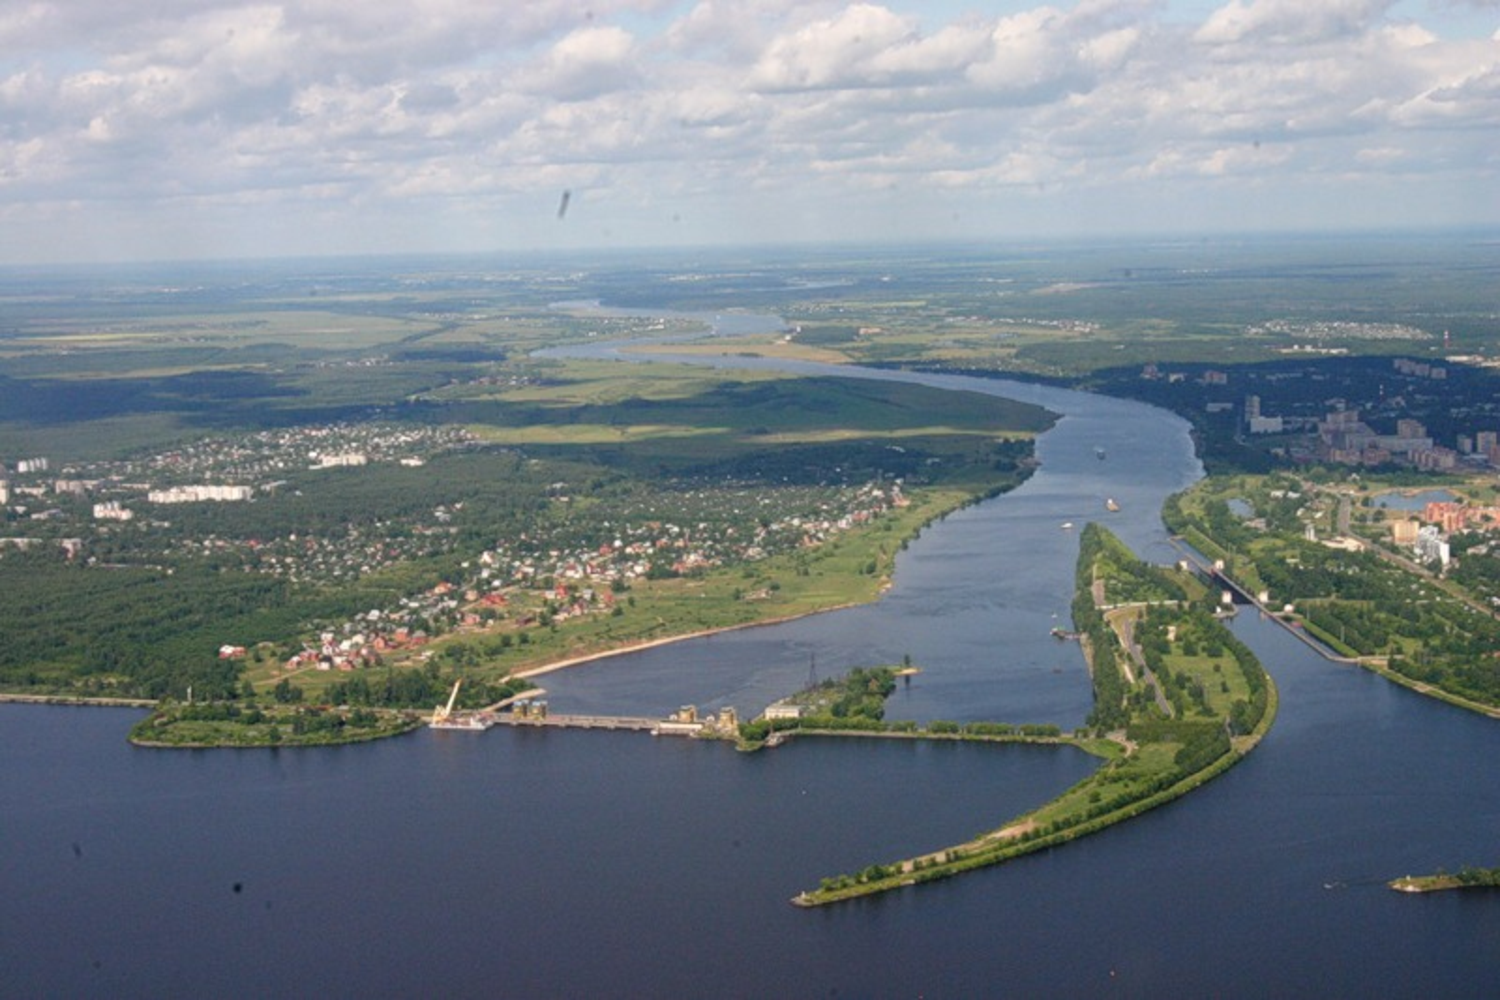
\includegraphics[scale=0.2]{dubna_town.pdf}}{}
\addtobeamertemplate{title page}{\centering 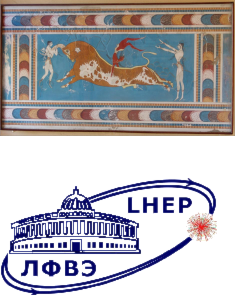
\includegraphics[scale=.4]{logos_2.png}}{} 
%\addtobeamertemplate{title page}{\centering 
\includegraphics[scale=0.095]{wpcf2018/wpcf2018_2.png}}{}

\title[\bf 7th International Conference on New Frontiers in Physics (ICNFP2018) ]{\textbf{\large {Studies of baryonic matter at BM@N}}}

%\author[P.~Batyuk]{\textit{\textbf{{\footnotesize \underline{P.~Batyuk}, L.~Malinina (SINP MSU, JINR), \\ O.~Rogachevskiy (JINR)}}} \\
%  on behalf of the MPD collaboration}
\author[\bf P.~Batyuk]{\textit{\textbf{{\footnotesize \underline{P.~Batyuk for BM@N Collaboration}}}}} 
%on behalf of the MPD collaboration} 
\institute{\bf Dubna, Joint Institute for Nuclear Research}
\vskip -.3cm
\date{{\textbf{Workshop on Physics at FAIR-NICA-SPS-BES/RHIC (July 10-11, 2018)}}}  
% \newpage \footnotesize April 14, 2016}}

\lstset{
  %    frame=tb, % draw a frame at the top and bottom of the code block
  tabsize=4, % tab space width
  showstringspaces=false, % don't mark spaces in strings
  %   numbers=left, % display line numbers on the left
  commentstyle=\color{blue}, % comment color
  keywordstyle=\color{blue}, % keyword color
  stringstyle=\color{red} % string color
}

\graphicspath{{wpcf2018/}}

\begin{document}
\maketitle

\begin{frame}
  \bf
  \frametitle{\bf \centering Outline}
  \begin{itemize}
  \item Nuclotron and physics to be investigated
  \item BM@N experiment
  \item Experimental results within the BM@N experiment
  \item Short Range Correlations program as an extension to the BM@N experiment
  \end{itemize}
\end{frame}

\begin{frame}
  \bf
  \frametitle{NICA Complex}
  \vskip -.75cm
  \begin{columns}[t]
    \column{.49\textwidth}
            {\footnotesize
    \begin{block}{}
      \begin{figure}[H]
        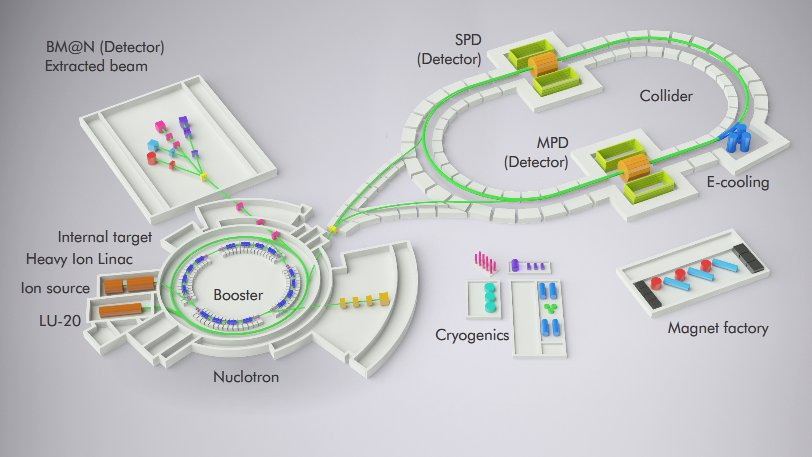
\includegraphics[width=1.\linewidth]{nica_complex1.png}
      \end{figure}
      %\centering The general contractor is  {\color{red} STRABAG} (Bodostal-3 \& PCJ are the sub-contractors)
    %\end{block}
    \vskip -.6cm

   % \begin{block}{}
      \begin{itemize}
      \item Set of accelerators providing particle beams for fixed target and collider experiments
      \item Experimental facilities
      \item Line for assembling and cryogenic testing of SC-magnets
      \item Workshops for construction of the detector elements
      \item NICA innovation center
      \end{itemize}
    \end{block}
        }
            \column{.49\textwidth}
            {\footnotesize 
              \begin{block}{}
      \centering  Beams - {\color{red}$p$, $d$ ... $^{197}Au^{79+}$} \\
      \centering  Collision energy: \\
        $\sqrt{s_{NN}}$ = {\color{red} 4 - 11} GeV,
        $T$ =  {\color{red}1 - 6} AGeV \\
      Luminosity: {\color{red}$10^{27}~cm^{-2}s^{-1}$} (Au), {\color{red}$10^{32}$}~(p) \\
 \end{block}
 \vskip -.3cm
 \begin{block}{}
      \begin{itemize}
      \item 2 interaction points - {\color{red}MPD} ({\color{blue} ICNFP2018, report of V. Kolesnikov}) and  {\color{red}SPD}
      \item Fixed target experiment -  {\color{red}BM@N}
      \end{itemize}
 \end{block}
 \vskip -.35cm
 \begin{block}{}
      \begin{itemize}
      \item {\color{red} 2018:} extracted beams of heavy ions (Ar, Kr) are available within the BM@N experiment
      \item {\color{red} 2020}: a first configuration of the MPD setup available.
      \item {\color{red} 2023}: commissioning of the fully designed NICA-complex is foreseen.	
      \end{itemize}
 \end{block}
 }
  \end{columns}
  \note{The NICA complex is being built in Dubna and is considered as a set of different accelerators
    to provide a beam to be used in fixed-target and collider experiments.
    Also, one of the main components of the complex is a line for assembling and cryogenic testing of
    superconducting magnets. It will provide different beam species up to gold ions in energy range
    $\sqrt{s_{NN}}$ = {\color{red} 4 - 11} GeV with a planned level of luminosity of order of $10^{27}~cm^{-2}s^{-1}$ for gold ions.
    The complex will have two points where two experiments will be located: MPD and SPD. Fixed-target program is in
    an active progress and is presented by BM@N experiment.}
\end{frame}

\begin{frame}
  \frametitle{\bf \centering Nuclotron (in operation since 1993)}
  \vskip -.75cm
  \begin{columns}[t]
    \column{.49\textwidth}
    \begin{block}{\bf \centering Modernized in 2010 - 2015}
      \bf 
      \resizebox{\columnwidth}{!}{%
        \begin{tabular}{| l | l |}
          \hline			
          Parameters & Nuclotron \\
          \hline
          type & SC synchrotron \\
          \hline 
          particles & $\uparrow$p, $\uparrow$d, nuclei \\
          \hline
          injection energy [MeV/u] & 5 ($\uparrow$p, $\uparrow$d), 570-685 (Au) \\
          \hline max. kin. energy [GeV/u] & 12.07 ($\uparrow$p), 5.62 ($\uparrow$d), 4.38 (Au) \\
          \hline
          magnetic rigidity [T $\cdot$ m] & 25 - 43.25 \\
          \hline
          circumference [m] & 251.52 \\
          \hline
          cycle for collider mode [s] & 1.5-4.2 (active), 5.0 (total) \\
          \hline
          vacuum [Torr] & $10^{-9}$ \\
          \hline
          intensity, Au [ions/pulse] & 1 $\cdot 10^{9}$ \\
          \hline
          % transition energy [GeV/u] & 7.0 \\
          %  \hline
          spill of slow extraction [s] & up to 10 \\
          \hline
        \end{tabular}
      }
    \end{block}
  %  \vskip -.3cm
    \begin{block}{\bf \centering Run55: Feb - Apr, 2018}
      \begin{figure}[H]
        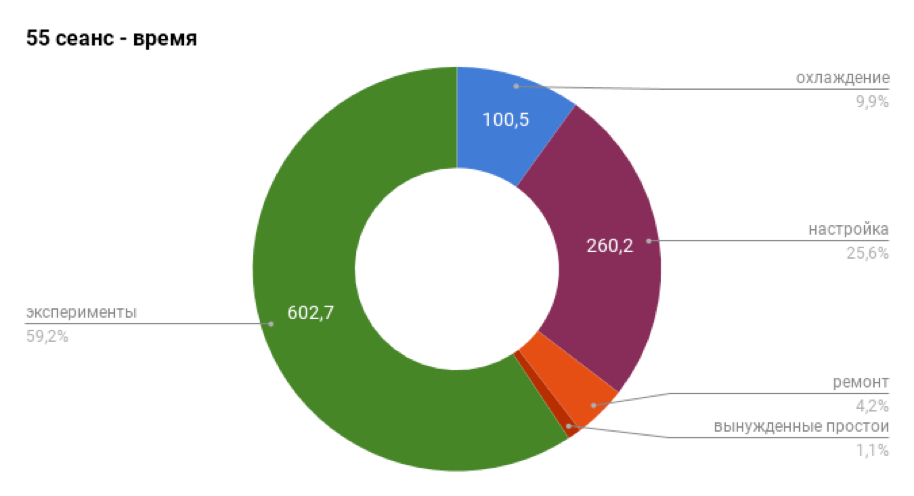
\includegraphics[width=1.\linewidth]{run55.png} \\
      \end{figure}
    \end{block}

    \column{.49\textwidth}
    \begin{block}{}
      \begin{figure}[H]
        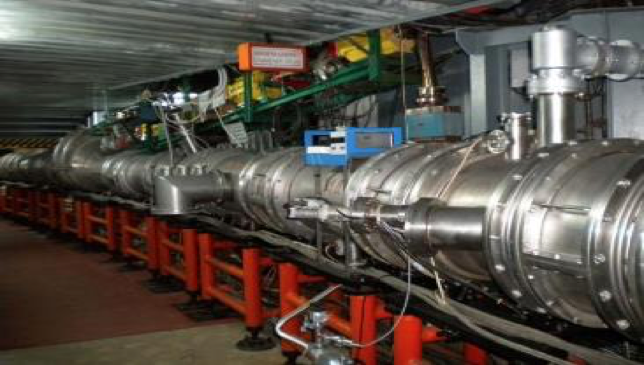
\includegraphics[width=1.\linewidth]{nuclotron1.png} \\
        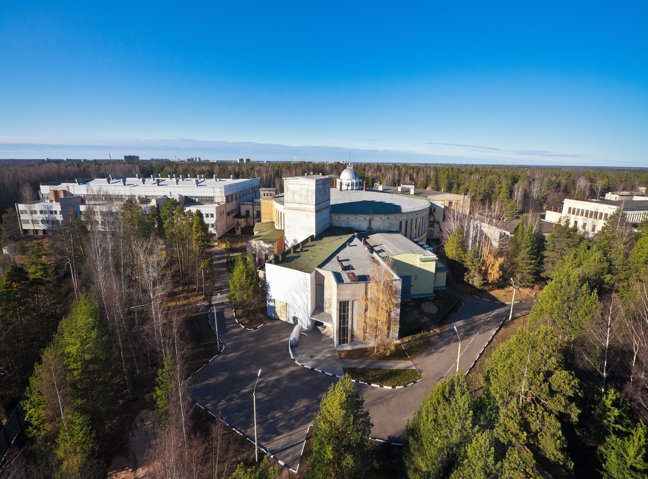
\includegraphics[width=1.\linewidth]{nuclotron2.png}
      \end{figure}
    \end{block}
  \end{columns}
  \note{The Nuclotron as a main accelerator of the complex is a synchrotron based on the SC magnets developed at JINR,
    was put in operation in 1993. In was essentially modernized in 2010-2015. It will provide acceleration of gold ions up to
    kinetic energy 4.4 GeV/u, and protons up to 12 GeV. In February we had an experimental run aimed at realizing
    fixed-target program within the BM@N experiment.}
\end{frame}

\begin{frame}
  \frametitle{\bf \centering BM@N experiment}
  \bf
       \vskip -.35cm
       \begin{columns}[c]
         \column{.69\textwidth}
         \begin{block}{\bf \centering Full setup, layout}
           \begin{figure}[H]
             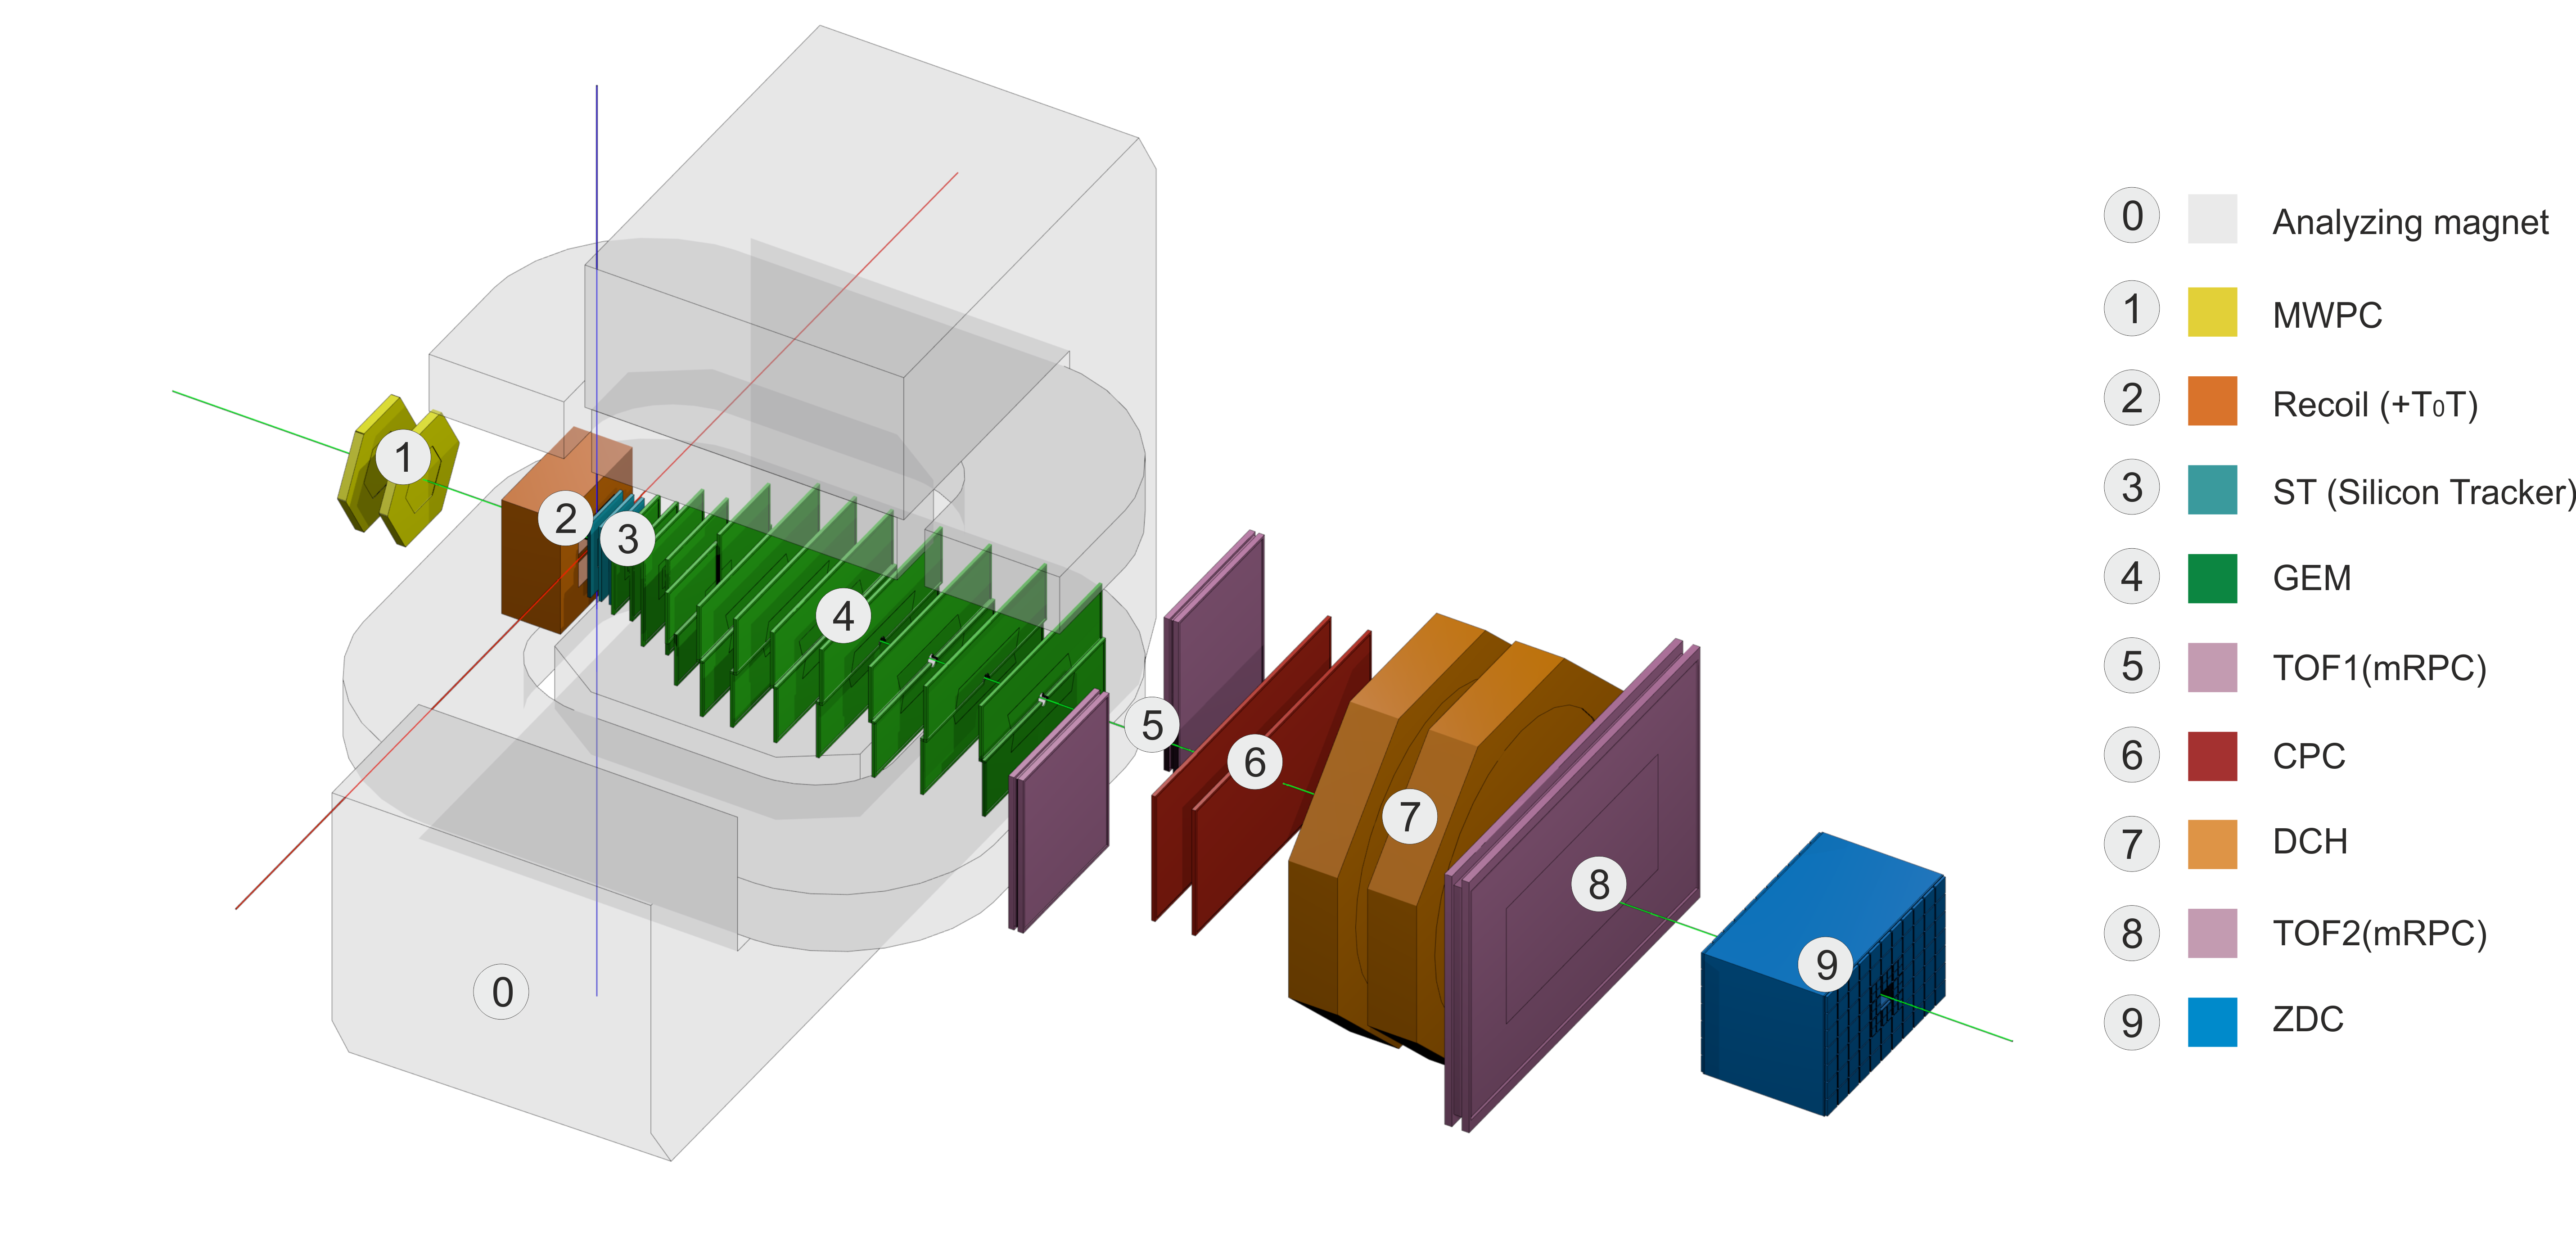
\includegraphics[width=1.\linewidth]{bmn_full_config_color_detectors_moreDarkMagnet_without_straw_labels.png}
           \end{figure}
         \end{block}

         \column{.29\textwidth}
         {\tiny
           \begin{block}{}
             \begin{itemize}
             \item Central tracker (Silicon tracker + GEM) inside analyzing magnet to reconstruct
               AA-interactions
             \item Outer tracker (CPC, DCH) behind magnet to link tracks from central tracker to ToF detectors
             \item TOF1 \& TOF2 system based on mRPC and T0 detectors to identify hadrons and light nuclei
             \item Detectors to form T0 and beam monitors
             \item ZDC calorimeter to measure centrality of AA-collisions
             \item Electromagnetic calorimeter for $\gamma$, $e^{+}$, $e^{-}$
             \end{itemize}
           \end{block}
         }
       \end{columns}
       \vskip -.2cm
       {\footnotesize
         \begin{block}{\bf \centering {\scriptsize  BM@N advantages:}}
           \vskip -.1cm
         \begin{itemize}
         \item \centering large aperture analyzing magnet
         \item sub-detector systems are resistant to high multiplicities of charged particles
         \item PID: "near to magnet" (TOF1), "far from magnet" (TOF2)
         \end{itemize}
       \end{block}
       }
\end{frame}

\begin{frame}
  \bf
  \frametitle{\bf \centering QCD phase diagram}
  \vskip -.75cm
  \begin{columns}[t]
    \column{.49\textwidth}
    \begin{block}{}
      \begin{figure}[H]
        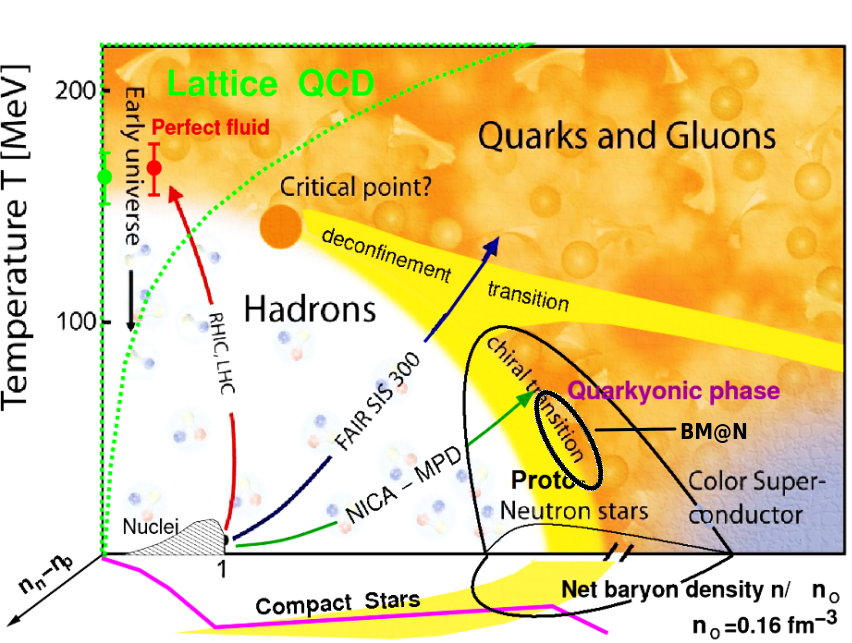
\includegraphics[width=1.\linewidth]{qcd_diagram.png}
      \end{figure}
    \end{block}
    \vskip -.75cm

    \begin{columns}[t]
      \column{.48\textwidth}  
      \begin{block}{\bf \centering {\tiny High energy:}}
        {\tiny
          \begin{itemize}
          \item $N_{baryons} \approx N_{antibaryons}$
          \item Lattice QCD predicts crossover transition between hadronic and partonic matter
          \item ALICE, ATLAS, CMS, STAR, PHENIX
          \end{itemize}
        }
      \end{block}
      \column{.48\textwidth}
      \begin{block}{\bf \centering {\tiny High net-baryon density:}}
        {\tiny
          \begin{itemize}
          \item $N_{baryons} >> N_{antibaryons}$
          \item Lattice QCD not applicable, models predict structures and exotic phases 
          \item BES @ RHIC, NA61, CBM, {\color{red} NICA/MPD, BM@N}
          \end{itemize}
        }
      \end{block}
    \end{columns}

    \column{.48\textwidth}
    \begin{block}{\bf \centering  Landscape of experiments exploring QCD phase diagram}
      \vskip .25cm
      \begin{figure}[H]
        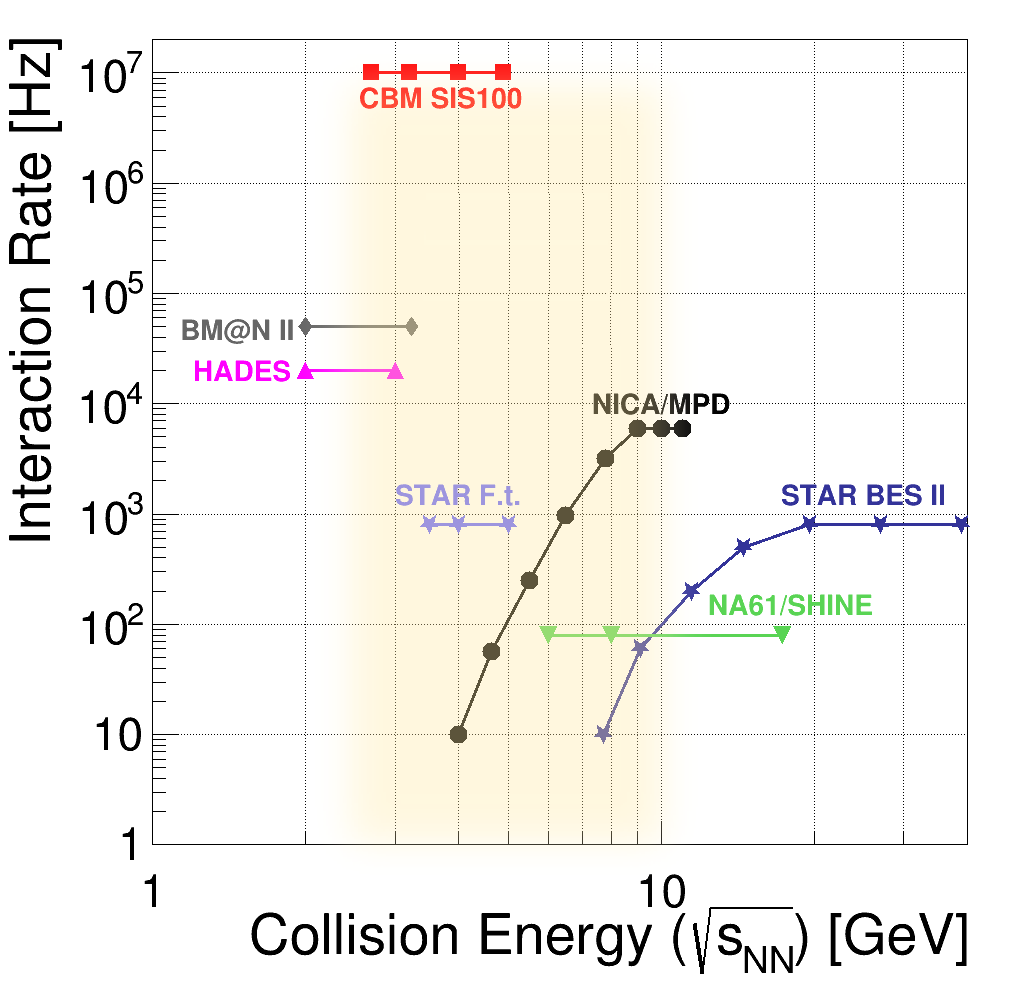
\includegraphics[width=1.\linewidth]{QCD_dense_matter_experiments.png}
      \end{figure}
    \end{block}
  \end{columns}
  \note{One of the most urgent task for the study of the QCD phase diagram is density frontier.
    According to various calculations maximum freeze-out density is reached at the energy range around $\sqrt{s_{NN}}$ = 10 GeV/n.
    So, NICA is well suited for exploring the transition between the hadronic and quark-gluon phases at the high net-baryon
    density. This is the top priority of the NICA program. \\
    The landscape of HIC experiments, present and future, in the energy
    region of max baryonic density are presented in this figure. Among fixed target experiments
    CBM at FAIR will provide maximum interaction rate. There are only two collider experiments – NICA and STAR BES with
    a difference in interaction rate of 3-4 orders of magnitude. Two NICA experiments - BM@N with fixed target and MPD
    at the collider will cover the whole indicated energy region.
  }
\end{frame}

\begin{frame}
  \bf
  \frametitle{\bf \centering {\footnotesize Exploring high density baryonic matter with Nuclotron}}
  \vskip -.75cm
  \begin{columns}[t]
    \column{.51\textwidth}
    \begin{block}{}
      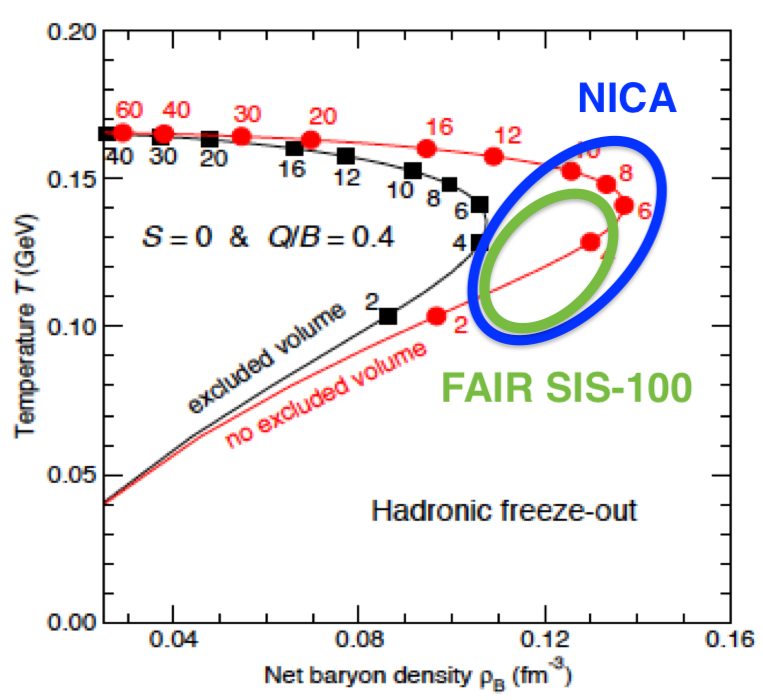
\includegraphics[width=1.\linewidth]{bar_densities.png}
    \end{block}
    \column{.47\textwidth}
       \begin{block}{}
         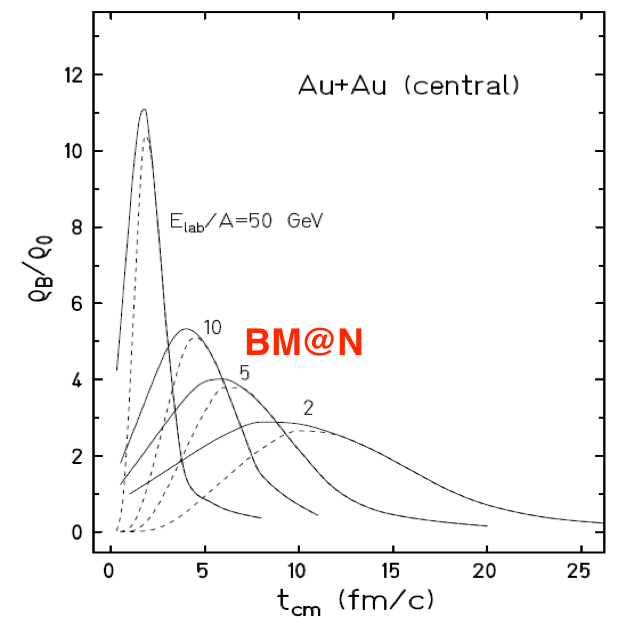
\includegraphics[width=1.\linewidth]{barDensDomination.png}
       \end{block}
\end{columns}
  \begin{block}{}
    \begin{center}
      Nuclotron is well suited to study high density (dominantly baryonic) matter since at that energies
      baryon-dominated system exists comparatively long lifetime
    \end{center}
  \end{block}
\end{frame}

\begin{frame}
  \bf
  \frametitle{Physics possibilities at the Nuclotron}
  % {\small
  \vskip -.75cm
               \begin{columns}[t]
                 \column{.49\textwidth} 
                 \begin{block}{\bf \centering $A+A$ collisions:}
                   \begin{itemize}
                   \item strangeness at threshold
                   \item Need more precise data for strange mesons, hyperons and hypernuclei, multi-variable distributions, unexplored energy range
                   \end{itemize}
                 \end{block}
                 \begin{block}{\bf \centering $p+p$, $p+n$, $p+A$ collisions:}
                   \begin{itemize}
                   \item Hadron production in elementary reactions and ``cold'' nuclear matter as a ``reference'' to determine exactly nuclear effects 
                   \end{itemize}
                 \end{block}
                 
                 \column{.44\textwidth} 
                 \begin{block}{\centering \bf {\color{yellow}{AGS}} {\color{red}{NA49}} {\color{ForestGreen}{BRAHMS}}}
                   %  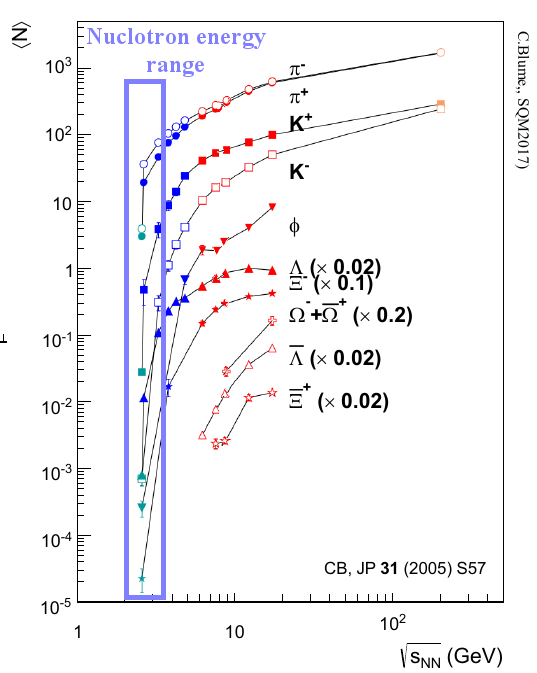
\includegraphics[width=.4\linewidth]{strangeness_prod.png}
                   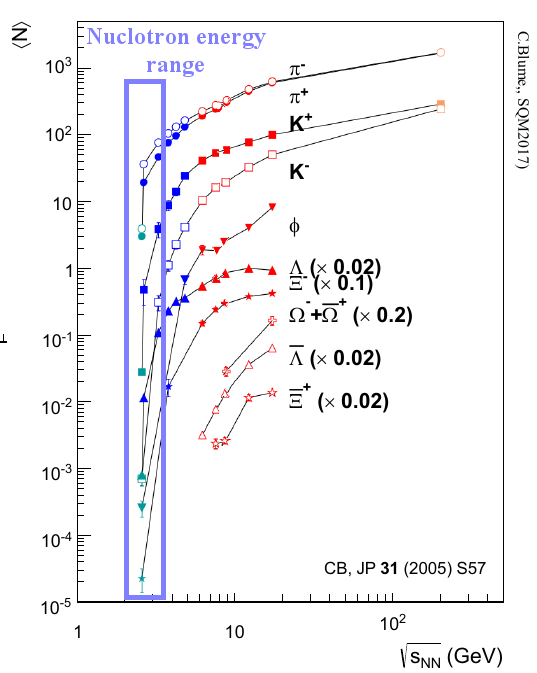
\includegraphics[width=1.\linewidth]{strangeness_prod.png}
                 \end{block}
                 %\begin{block}{}
                  % 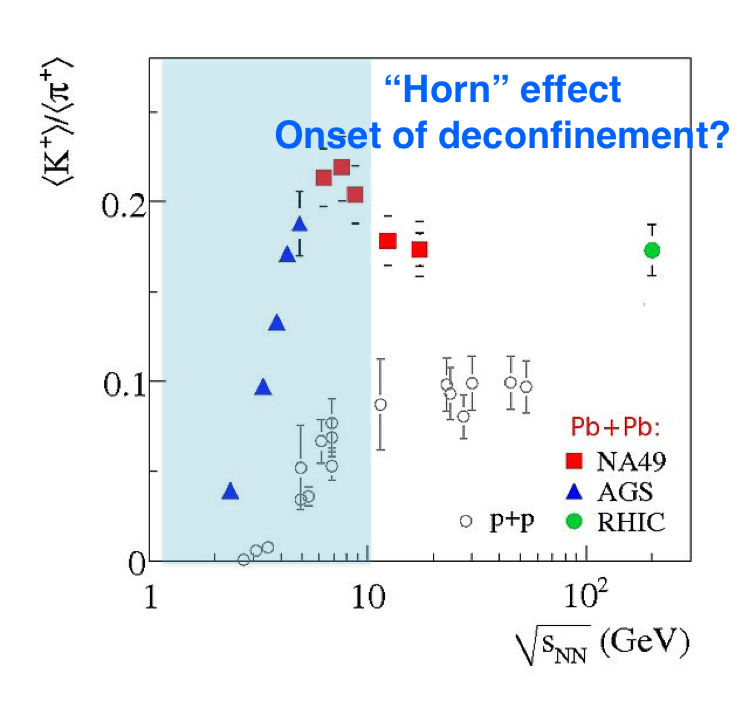
\includegraphics[width=1.\linewidth]{horn_NA49.png}
                 %\end{block}
               \end{columns}
               %  }
               \note{Production of strange particles in A+A collisions is of particular interest because their
                 enhanced yields (relative to pp reactions) have been predicted as the signal of the deconfinement phase
                 transition. Such enhancement, indeed, was observed at SPS energies and then confirmed at the RHIC.
                 However, the data on strangeness production, especially at threshold, at energy region of the maximum baryonic
                 density are not complete or even missing}
\end{frame}

\begin{frame}
  \bf
  \frametitle{Heavy ions $A+A$: Hypernuclei production}
  \vskip -.75cm
  \begin{columns}[t]
    \column{.49\textwidth}
    \begin{block}{{\tiny \bf \centering A. Andronic et al., Phys. Lett. B697 (2011) 203}}
      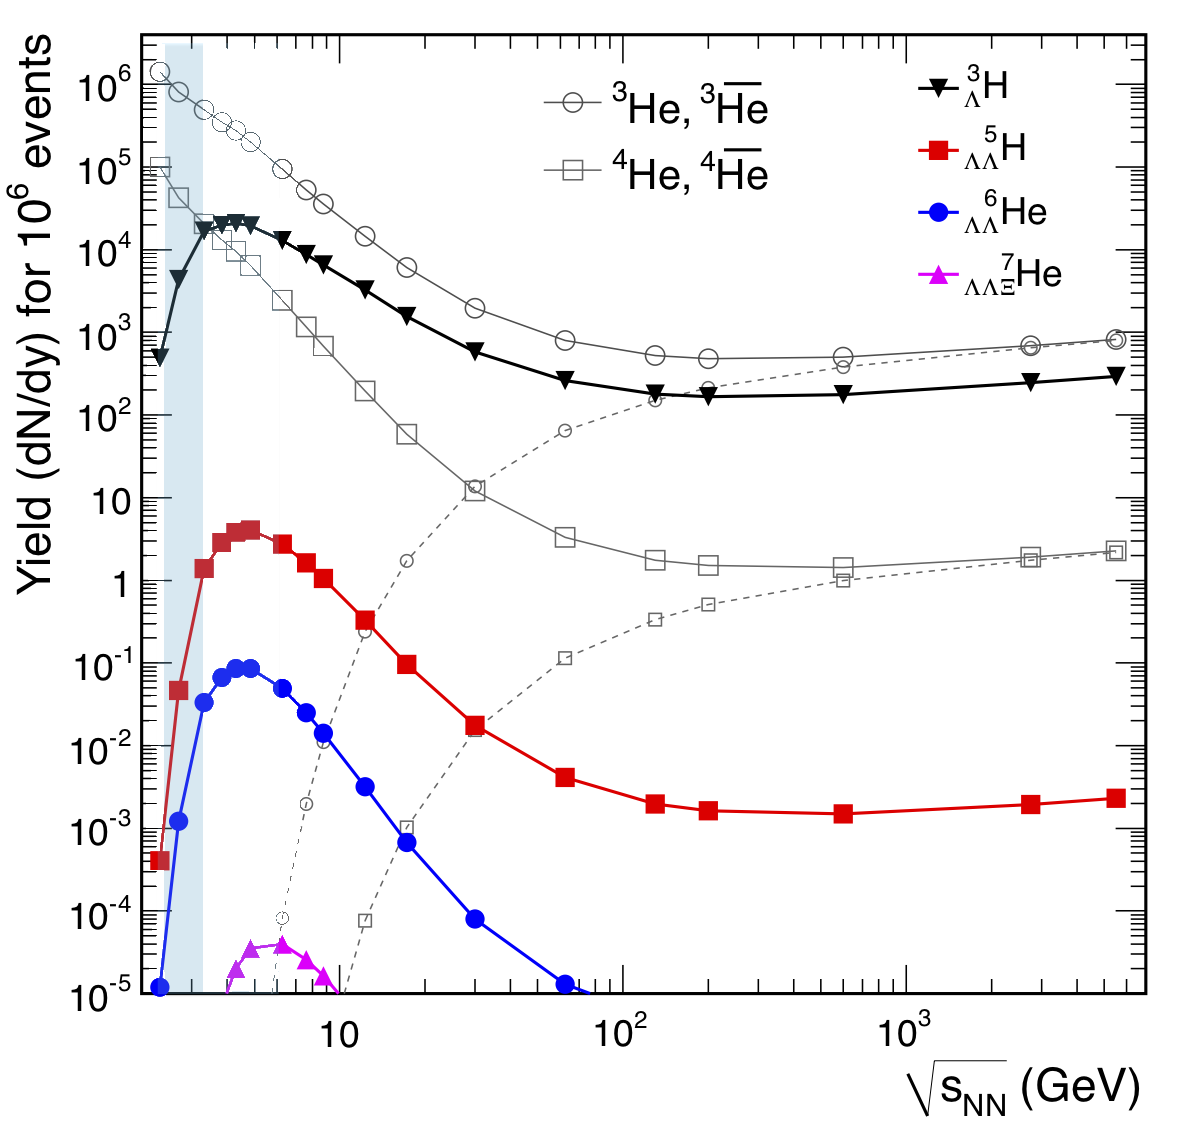
\includegraphics[width=1.\linewidth]{hypernucl_prod.png}
    \end{block}
    \vskip -.2cm
    \begin{block}{}
    \centering 
        {\color{ForestGreen} BM@N energy range} is {\color{red} suited} for the search of (double) hypernuclei
  \end{block}
    \column{.49\textwidth}
    \begin{block}{}
      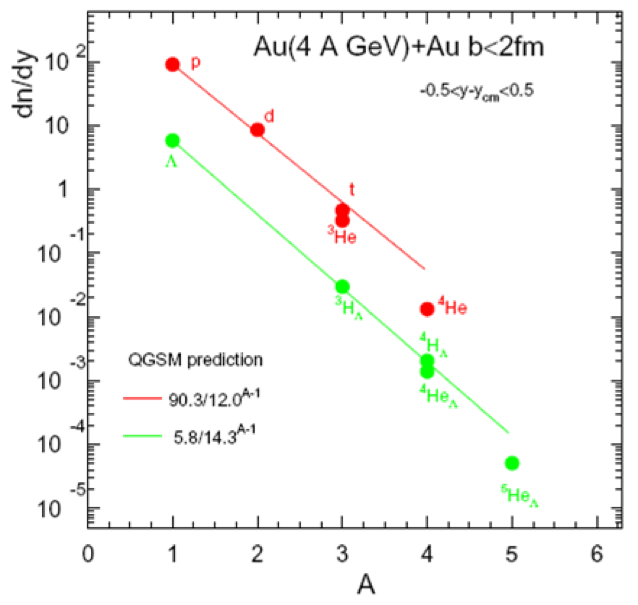
\includegraphics[width=1.\linewidth]{dNdY_asAdep.png}
    \end{block}
    \vskip -.3cm
    {\scriptsize
      \begin{block}{}
        \vskip -.1cm
       \begin{itemize}
      \item {\color{red} In heavy-ion collisions:} production of hypernuclei through coalescence of $\Lambda$
        with light fragments enhanced at high baryon densities
      \item {\color{red} Maximal yield} predicted for $\sqrt{s_{NN}}$ = 4 - 5~AGeV (stat. model)
        %(interplay of $\Lambda$ and light nuclei excitation function)
     \end{itemize}
     \end{block}
     }
  \end{columns}
  \note{Hypernuclei provide unique opportunity to study hyperon-nucleus interactions in a many-body environment.
    Details of the strange sector in the nuclear matter equation-of-state (EOS) are of great importance for astrophysics
    and should help understanding the mechanism of creation and evolution of super-dense stellar objects - neutron stars.
    Results of model calculations indicate, the yields of hypernulei in central heavy ion collisions are enhanced within
    the NICA energy range, this gives good perspectives for such kind of studies at NICA.}
\end{frame}

\begin{frame}
  \bf
  \frametitle{\bf \centering {\footnotesize BM@N feasibility study, GEM tracker performance}}
  
 % \begin{columns}[t]
 %   \column{.4\textwidth}
  % \begin{block}{\bf \centering {\scriptsize Acceptance for primary photons, mom. resolution, det. efficiency}}
  \begin{center}
    \vskip -.5cm
           {\bf \footnotesize \centering Acceptance for primary photons, mom. resolution, det. efficiency}
  \end{center}
  \begin{center}
      \begin{minipage}{.49\linewidth}
        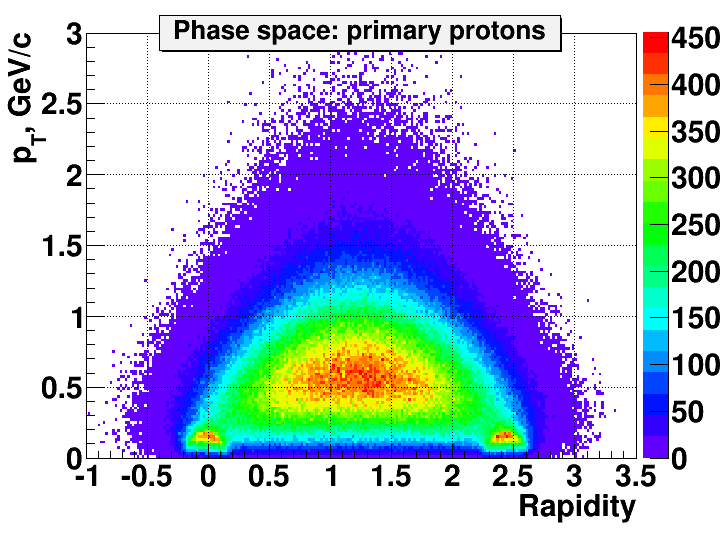
\includegraphics[width=.9\linewidth]{phaseSpace_sim.png} 
        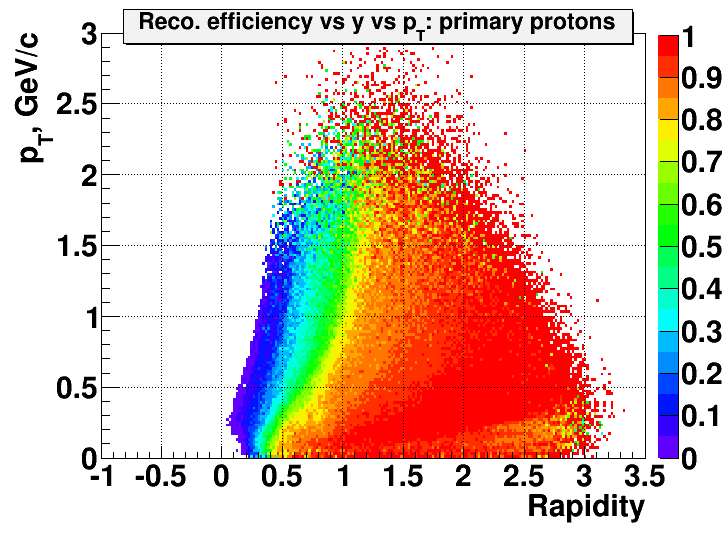
\includegraphics[width=.9\linewidth]{phaseSpace_reco.png}
      \end{minipage}
      \begin{minipage}{.49\linewidth}
        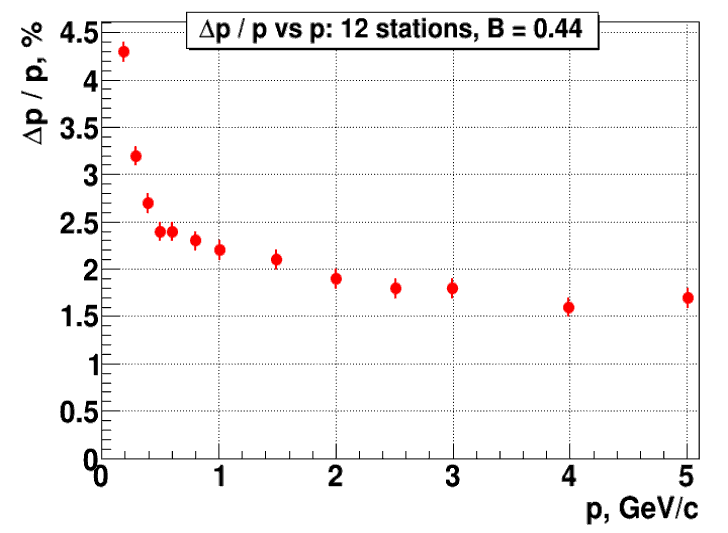
\includegraphics[width=.9\linewidth]{momRes_GEM.png} 
        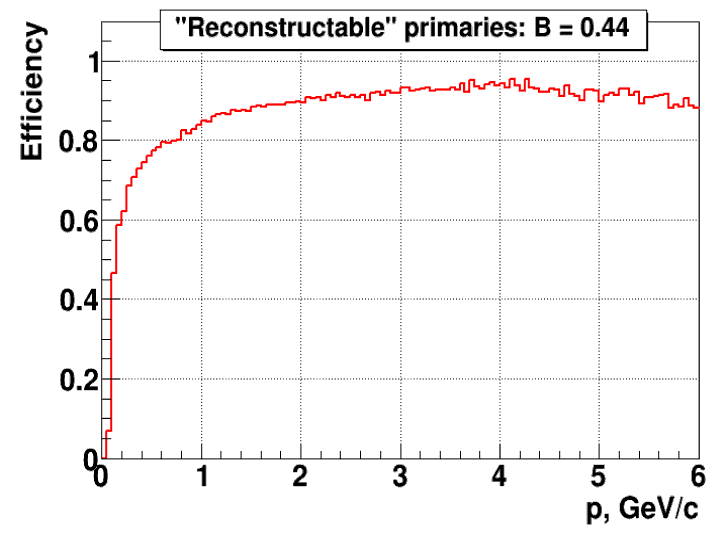
\includegraphics[width=.9\linewidth]{eff_GEM.png}
      \end{minipage}
  \end{center}
%\end{block}
 %   \column{.4\textwidth}
 %   \begin{block}{\bf \centering {\scriptsize Mom. resolution / det. efficiency}}
 %     \begin{minipage}{1.\linewidth}
       
 %     \end{minipage}
 %   \end{block}   
%  \end{columns}
\end{frame}

\begin{frame}
  \bf
  \frametitle{\bf \centering {\footnotesize BM@N feasibility study, strangess and hypernuclei}}
  \vskip -.3cm
   \begin{block}{}
      Simulation: UrQMD \& DCM-QGSM, Au+Au,  T = 4.5 AGeV
   \end{block}
   \vskip -.5cm
  \begin{columns}[t]   
    \column{.49\textwidth}
    \begin{block}{}
      \begin{center}
      900k central events, \\
      7.5M  $\Xi^{-}$ in 1 month \\
      20 kHz trigger
      \end{center}
    \end{block}
    \vskip -.2cm
    \begin{block}{}
       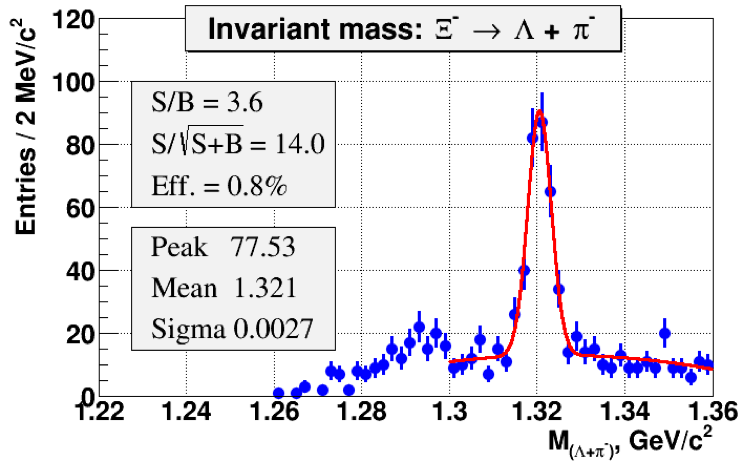
\includegraphics[width=1.\linewidth]{BMN_ksi.png}
    \end{block}
    \column{.49\textwidth}
    \begin{block}{}
      \begin{center}
      2.6M central events, \\
      8.5M  \ce{^{3}_{$\Lambda$}H} in 1 month \\
      20 kHz trigger
      \end{center}
    \end{block}
    \vskip -.2cm
     \begin{block}{}
       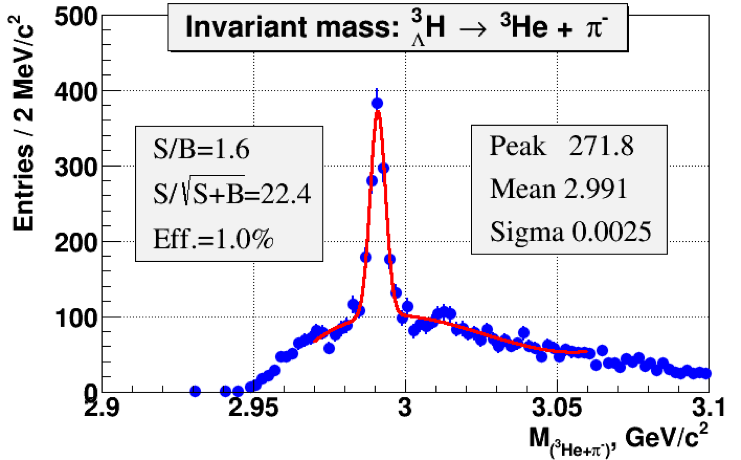
\includegraphics[width=1.\linewidth]{BMN_hyperTrit.png}
    \end{block}
  \end{columns}
  \begin{block}{}
    \begin{center}
      \bf The feasibility study indicates reliable reconstruction of cascades and hypernuclei of order of 10 millions per month
    \end{center}
    \end{block}
  \note{}
\end{frame}

\begin{frame}
  \bf
  \vskip -.8cm
  \frametitle{\bf \centering Data processing for offline Event Display}
  \begin{columns}[t]
    \column{.3\textwidth}
    \begin{block}{\bf \centering {\footnotesize Sim \& Reco}}
      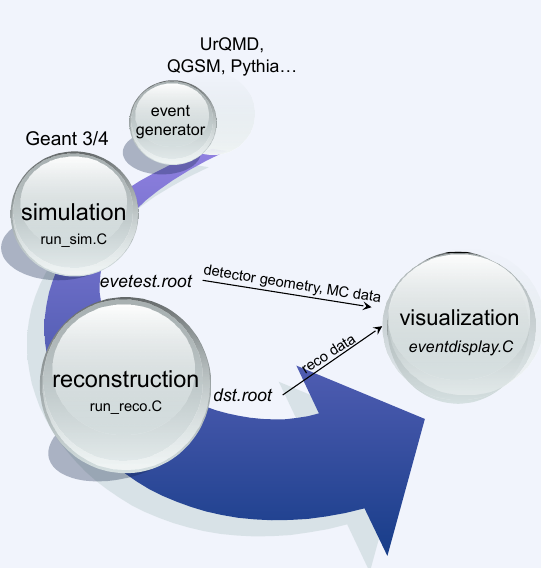
\includegraphics[width=1.\linewidth]{offline_anal.png}
  %  \end{block}
  %  \vskip -.3cm
  %  \begin{block}{\bf \centering {\footnotesize Reco}}
      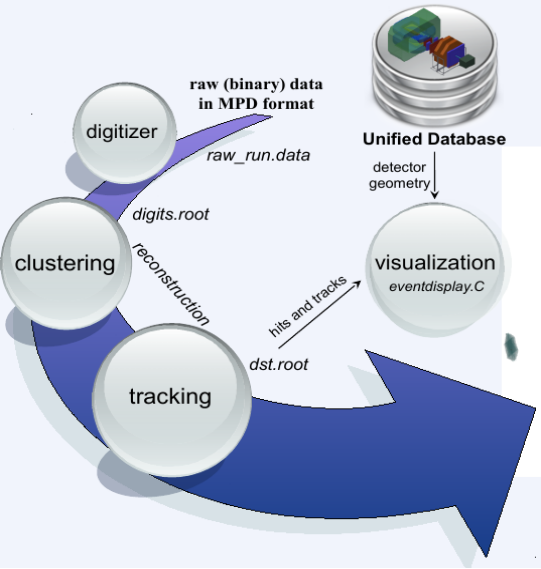
\includegraphics[width=1.\linewidth]{offline_anal_v2.png}
    \end{block}
    
    \column{.59\textwidth}
    \begin{block}{}
      %\vskip -.2cm
      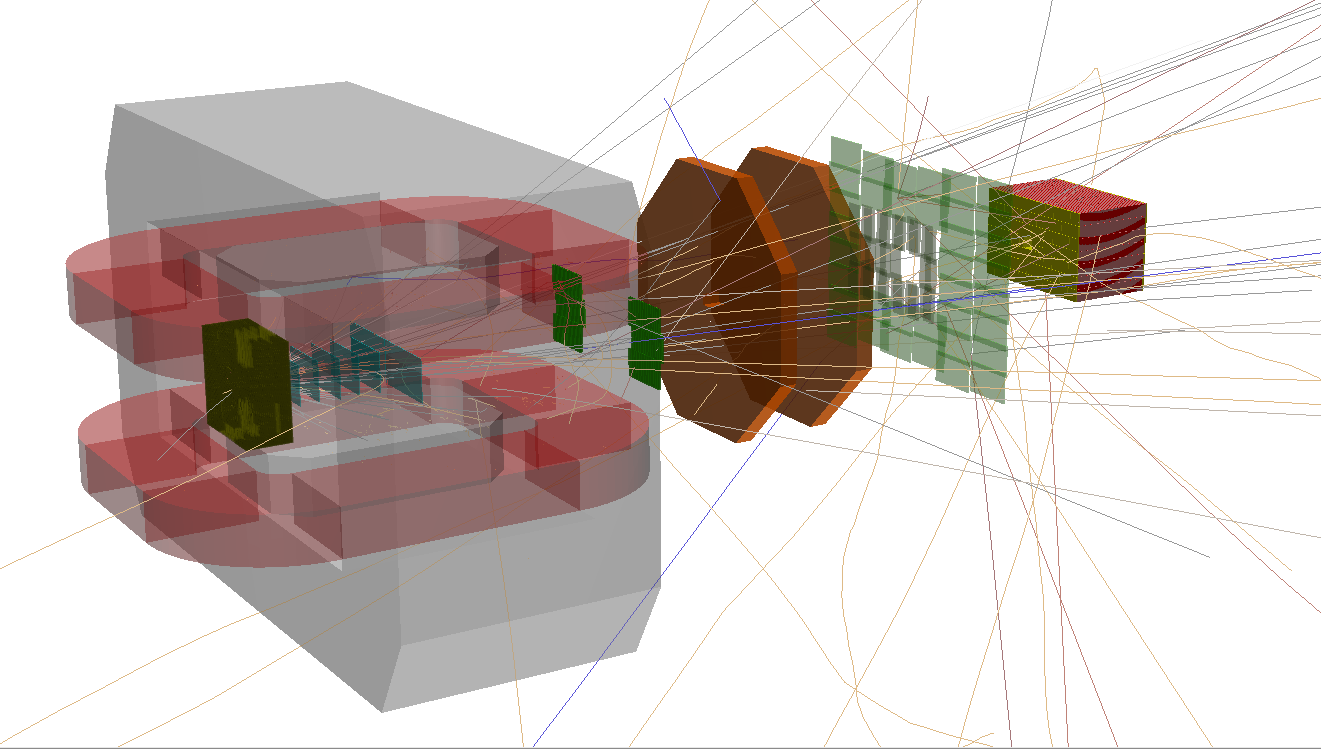
\includegraphics[width=1.\linewidth]{eventDisplay_run6_v2.png}
     % \vskip -.2cm
   % \end{block}
   % \begin{block}{}
    %  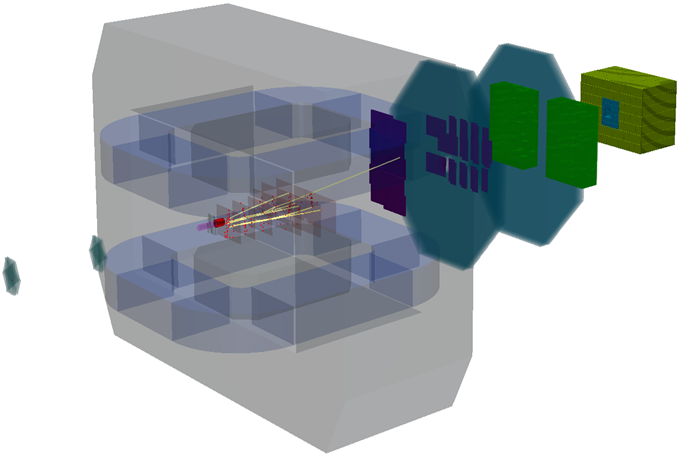
\includegraphics[width=1.\linewidth]{eventDisplay_run6_v3.png}
    \end{block}
    \vskip -.4cm
    {\footnotesize 
    \begin{block}{}
      \begin{itemize}
      \item The Event Display has been developed for graphical representations of the NICA experiments in offline as well as online mode and integrated into the
        BmnRoot software.
      \item The visualization system gives an opportunity to visually check the developed algorithms for reconstruction and physical analysis of data.
      \end{itemize}
    \end{block}
    }
    
  %\begin{columns}[t]
  %  \column{.49\textwidth}
  %   \begin{block}{}
  %    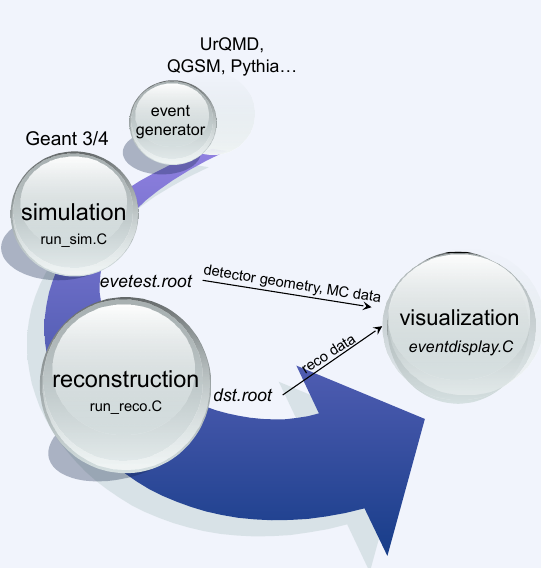
\includegraphics[width=1.\linewidth]{offline_anal.png}
  %   \end{block}
  %  \column{.49\textwidth} 
  \end{columns}
\end{frame}

\begin{frame}
  \bf
  \begin{block}{}
    \begin{center}
      {\Huge Some experimental results from deuteron and carbon runs}
    \end{center}
  \end{block}
\end{frame}

\begin{frame}
  \bf
  \frametitle{\bf \centering Setup \& Experimental program to be performed}
  \vskip -.1cm
 % \begin{block}{\bf \centering Setup:}
    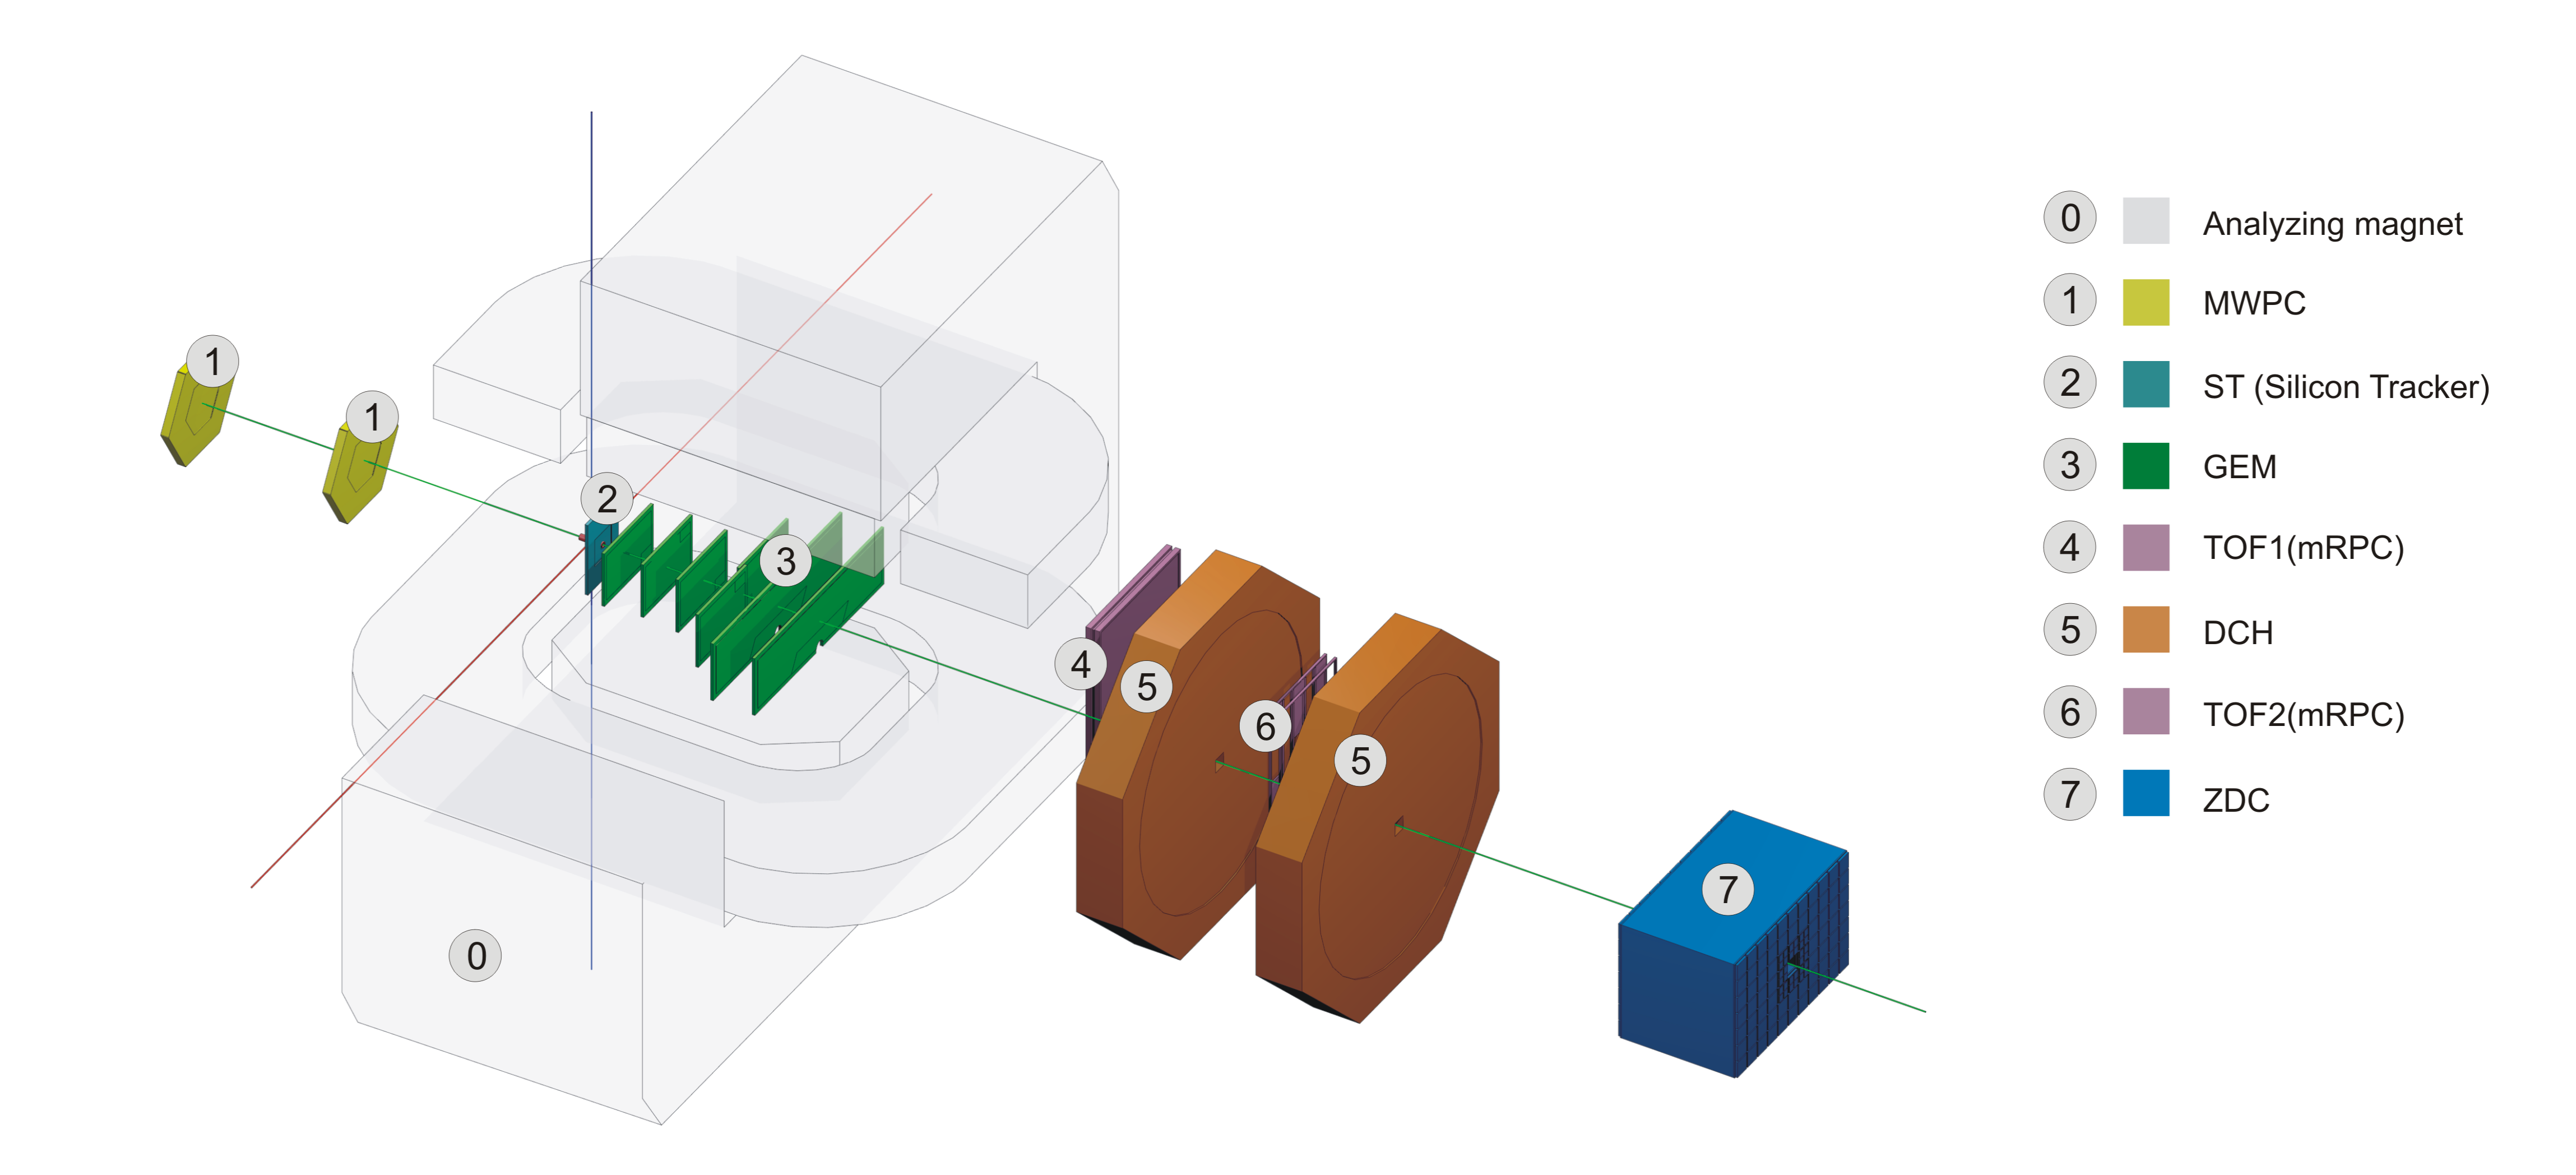
\includegraphics[width=1.\linewidth]{bmn_winter2016_config_common_view_labels.png}
 % \end{block}
  \vskip -.7cm
  {\tiny
  \begin{columns}[t]
    \column{.23\textwidth}
    \begin{block}{\bf \centering {\scriptsize Input beams:}}
      Deuteron beam (d), $T= 4.0, 4.6$ AGeV \\
      Carbon beam (C), $T = 3.5, 4.0,  4.5$ AGeV
    \end{block}
    \column{.33\textwidth}
    \begin{block}{\bf \centering {\scriptsize Aims:}}
      \begin{itemize}
      \item Focus on tests and commissioning  of central tracker inside analyzing magnet $\rightarrow$ GEM detectors and forward Si detector for tracking
      \item Test / calibrate ToF, trigger detectors, calorimeters
      \end{itemize}
    \end{block} 

    \column{.33\textwidth}
    \begin{block}{\bf \centering {\scriptsize Program:}}
      \begin{itemize}
      \item Trace beam through detectors, align detectors, measure beam momentum in mag. field of 0.3 - 0.85 T
      \item Measure inelastic reactions d (C) + target $\rightarrow$ X  with deuteron and carbon beam energies of 3.5 - 4.6 GeV/n on targets $CH_{2}$, C, Al, Cu, Pb
      \end{itemize}
    \end{block}
  \end{columns}
  }
\end{frame}

\begin{frame}
  \bf
  \vskip -.80cm
  \frametitle{\bf \centering \footnotesize Beam momentum measured with GEM tracker in carbon run}
  \begin{columns}[t]
    \column{.4\textwidth}
    \begin{block}{\bf \centering {\footnotesize $p$ vs. field current}}
       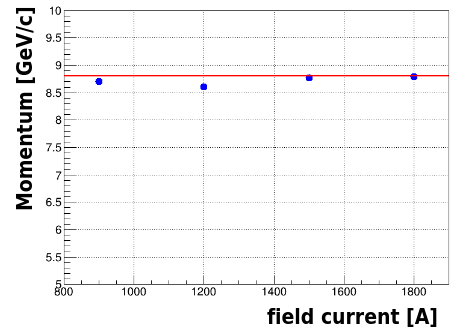
\includegraphics[width=1.\linewidth]{momBeam_run6.png}
    \end{block}
    \vskip -.4cm
    \begin{block}{\bf \centering {\footnotesize $\Delta p / p$ vs. field current}}
       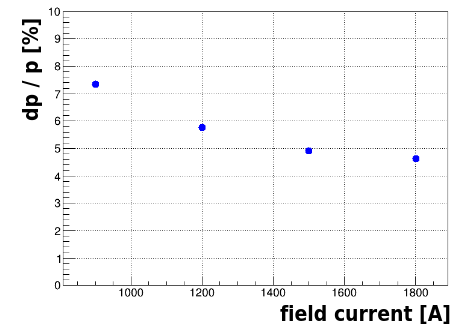
\includegraphics[width=1.\linewidth]{momResBeam_run6.png}
    \end{block}
    \column{.55\textwidth}
    \begin{block}{}
      \begin{itemize}
      \item Reconstruction of carbon beam trajectory and momentum in GEM detectors  at different values of magnetic field
      \item Gas mixture: Ar + $CO_{2}$ (70:30)
      \item Carbon beam run, T = 3.5 AGeV
      \end{itemize}
    %\end{block}
      % \begin{block}{}
      \vskip -.1cm
      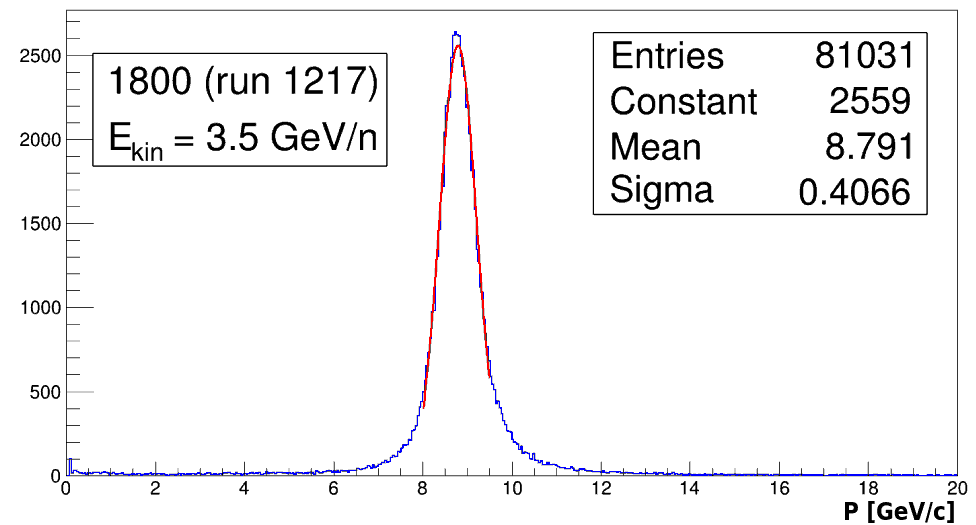
\includegraphics[width=1.\linewidth]{rigidity_1800A_run6.png}
    \end{block}
  \end{columns}
\end{frame}

\begin{frame}
  \vskip -.8cm
  \frametitle{\bf \centering  {$\Lambda^{0}$ in deutron and carbon runs}}
  \begin{columns}[t]
    \column{.35\textwidth}
    {\footnotesize 
     \begin{block}{}
       \bf
       \begin{center}
       d (C) + target $\rightarrow$ X \\
       $\Lambda^{0}$-signal width $\sim$ 2.5-3 MeV
       \end{center}
     \end{block}
    % \vskip -.3cm
    % \begin{block}{}
    %   \begin{center}
    %     {\color{red} \bf No detailed PID used}
    %   \end{center}
    % \end{block}
     }
    % \vskip -.3cm
     \begin{block}{\bf \centering {\footnotesize Deuteron run}}
       \begin{figure}[H]
         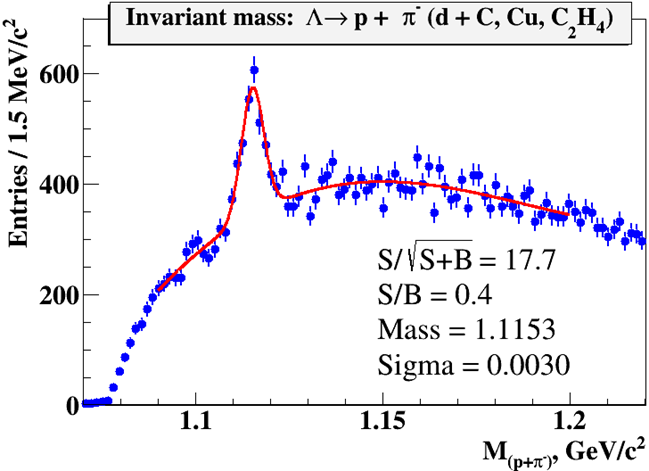
\includegraphics[width=1.\linewidth]{lambda_run5.png} 
       \end{figure}
     \end{block}
    \column{.60\textwidth}
    \begin{block}{\bf \centering {\footnotesize Carbon run, T = 4 AGeV}}  
      \begin{minipage}{.49\linewidth}
        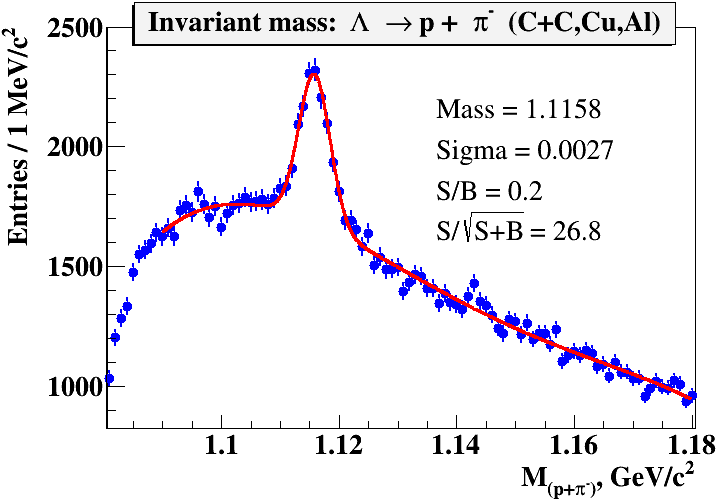
\includegraphics[width=1.\linewidth]{lambda_all.png}
        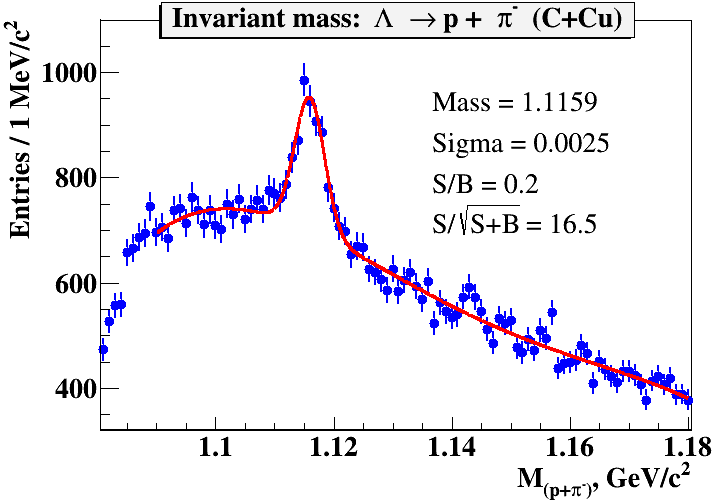
\includegraphics[width=1.\linewidth]{lambda_Cu.png}
      \end{minipage}
      \begin{minipage}{.49\linewidth}
        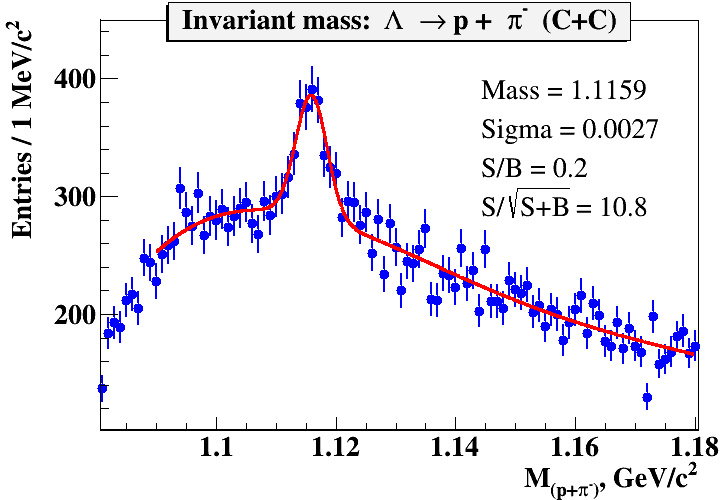
\includegraphics[width=1.\linewidth]{lambda_C.png}
        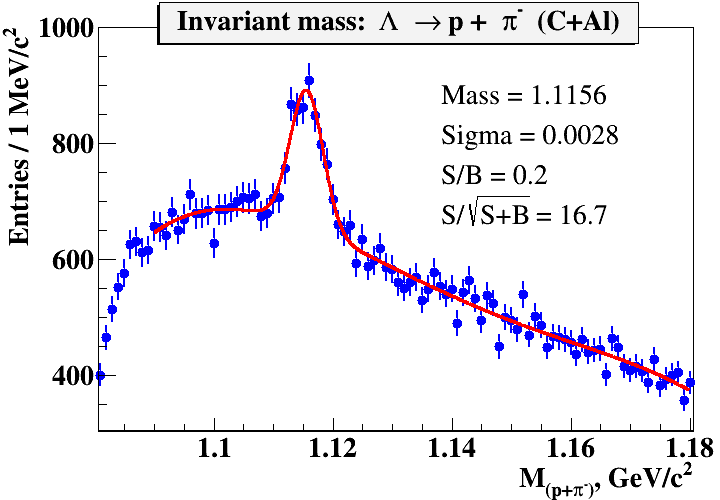
\includegraphics[width=1.\linewidth]{lambda_Al.png}
      \end{minipage}
    \end{block}
  \end{columns}
  \vskip -.3cm
  \begin{columns}[t]
    \column{.29\textwidth}
    \begin{block}{}
      \vskip -.1cm
      \bf
      {\footnotesize {\color{blue} PEPAN Lett., v.15, p.136, 2018(2):} {\color{red} First results from BM@N technical run with deuteron beam}}
    \end{block}
    \column{.68\textwidth}
   \begin{block}{}
     \bf
     {\scriptsize To improve vertex and momentum resolution and reduce background under $\Lambda^{0}$:
       \begin{itemize}
       \item Need few planes of forward Silicon detectors $\rightarrow$ 3 planes used in last run
       \item Need more GEM planes to improve track momentum reconstruction
       \end{itemize}
     }
   \end{block}
   \begin{block}{}

   \end{block}
   \end{columns}
\end{frame}

\begin{frame}
  \bf
  \frametitle{\bf \centering {\footnotesize TOF1 and TOF2 based on mRPC}}
 \vskip -.8cm
  \begin{columns}[t]
    \column{.49\textwidth}
  %  \begin{minipage}{1.\linewidth}
     \begin{block}{\bf \centering {\scriptsize AuAu @ T = 3.4~AGeV, $\pi^{\pm}$, 4m from target}}
       \begin{figure}[H]
         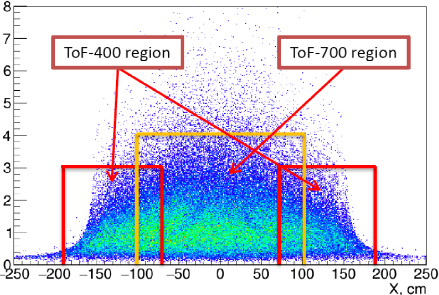
\includegraphics[width=1.\linewidth]{TOFs_simulation.png}
       \end{figure}
     \end{block}
    \vskip -.3cm
     %  \begin{minipage}{.45\linewidth}
     %  \begin{block}{\bf \centering {\scriptsize TOF2 wall} }
     %    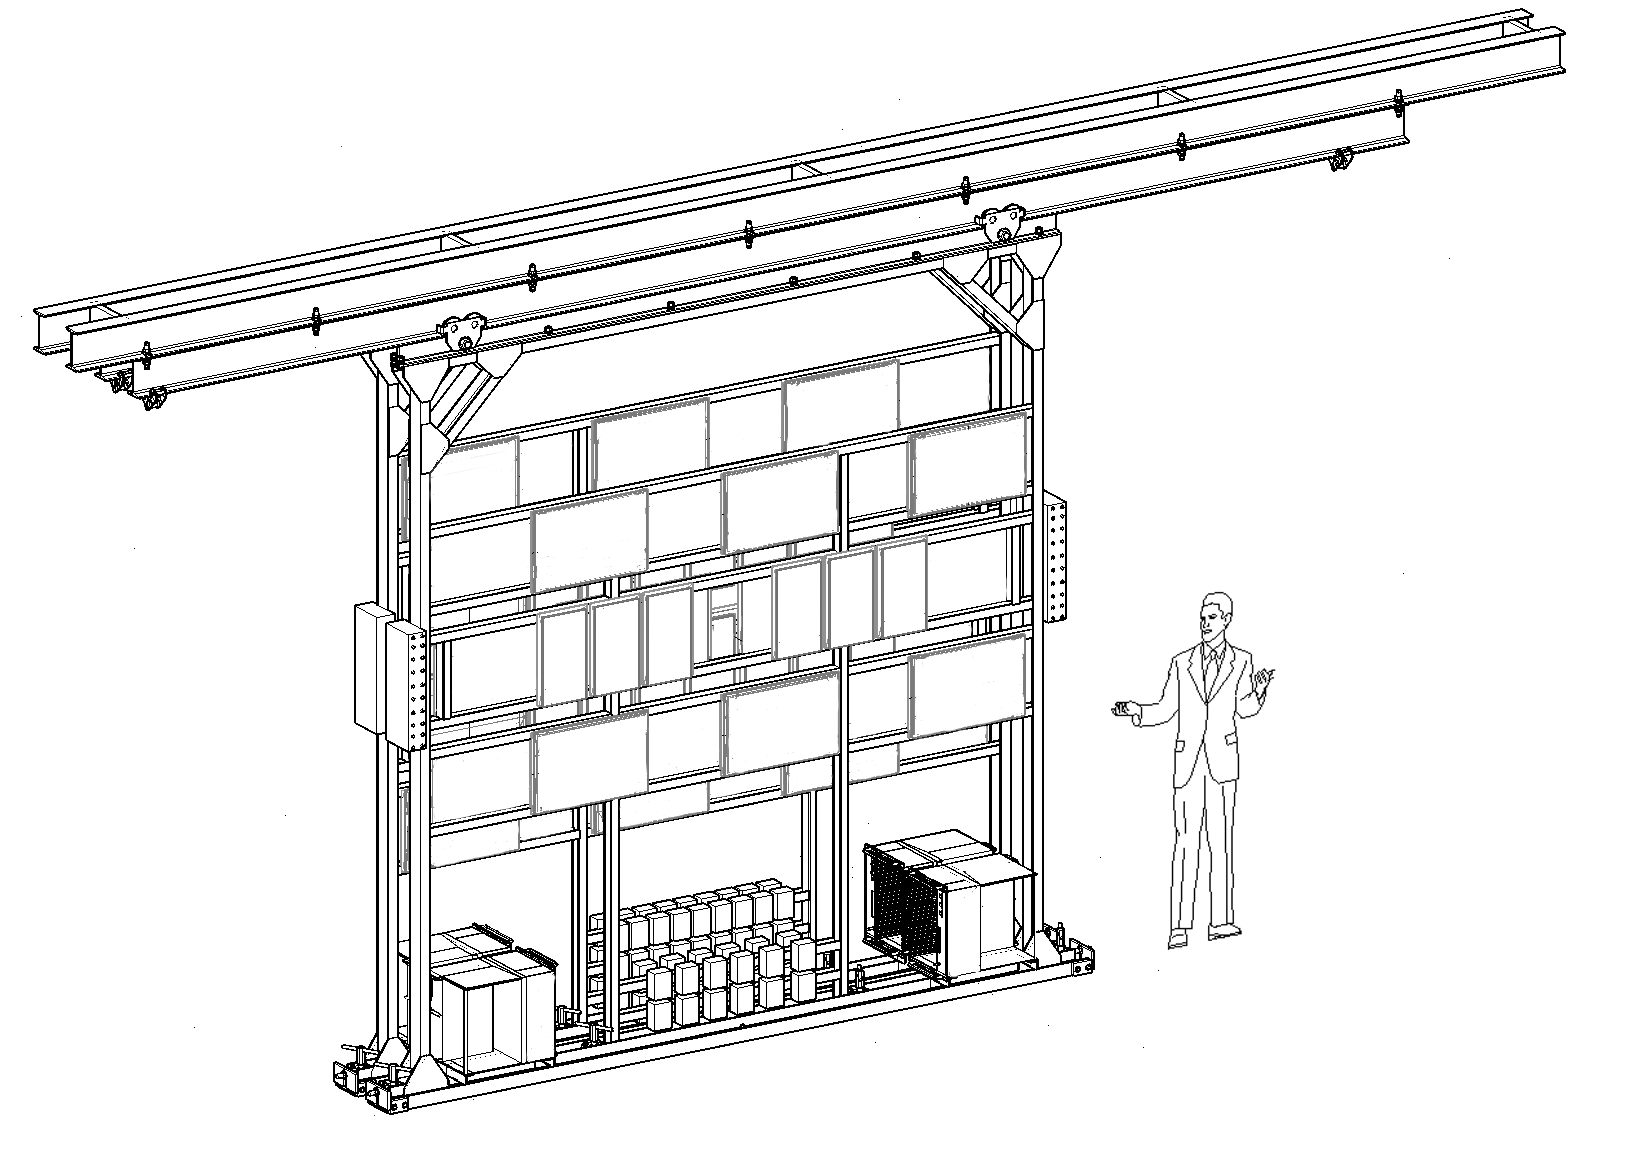
\includegraphics[width=1.\linewidth]{tof700_wall.png}
     %    \end{block}
    %  \end{minipage}
    {\footnotesize 
    \begin{block}{\bf \centering {\footnotesize Requirements to TOF system:}}
      \begin{itemize}
      \item high granularity to keep the overall system occupancy below 15\% and minimize efficiency degradation due to double hits
      \item operation at high particle flux
      \end{itemize}
    \end{block}
    }
  
    \column{.49\textwidth}
    % \begin{minipage}{1.\linewidth}
    \begin{block}{\bf \centering {\scriptsize Separation of $\pi / K$ for different time resolution and bases}}
       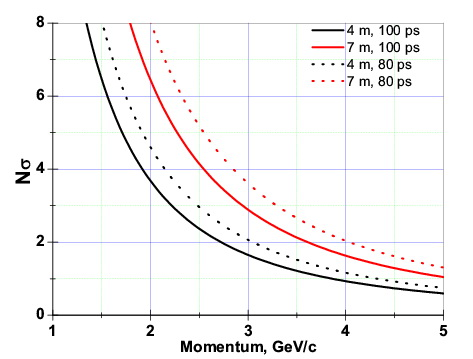
\includegraphics[width=1.\linewidth]{Nsigma_Pmom.jpg}    
    \end{block}
    \vskip -.3cm
   % \begin{block}{}
   %  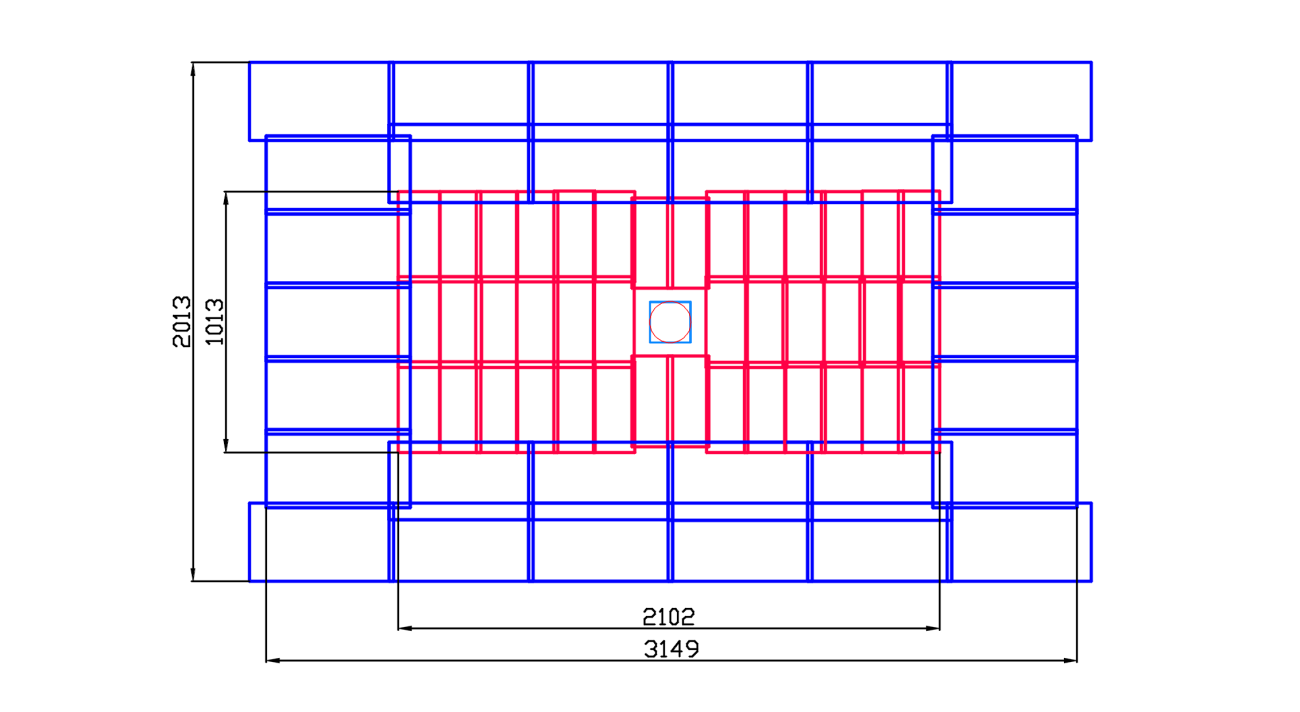
\includegraphics[width=1.\linewidth]{tof700_geo.png}
    %\end{block}
    {\footnotesize
    \begin{block}{}
      \begin{itemize}
      \item time resolution better then 80 ps
       \item high combined geometrical and detection efficiency (better than 95\%)
      
       \end{itemize}
    \end{block}
    }
  \end{columns}
\end{frame}


\begin{frame}
  \frametitle{\bf \centering TOF1 and TOF2 performance in carbon run}
  \begin{columns}[t]
    \column{.44\textwidth}
    \vskip -.82cm
    \begin{block}{\bf \centering {\scriptsize T = 3.5 GeV/n, C + Al $\rightarrow$ X}}
      {{\bf \centering \tiny Includes inf. from GEM tracking}}
      \vskip -.35cm
      \begin{figure}[H]
        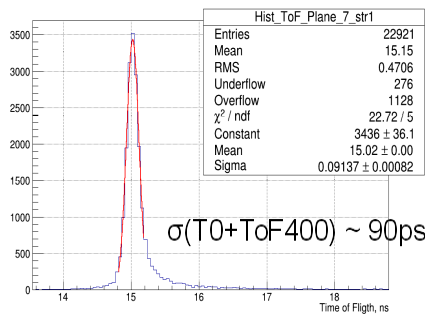
\includegraphics[width=1.\linewidth]{tof400_res.png}
      \end{figure}
      \vskip -.75cm
      \begin{figure}[H]
        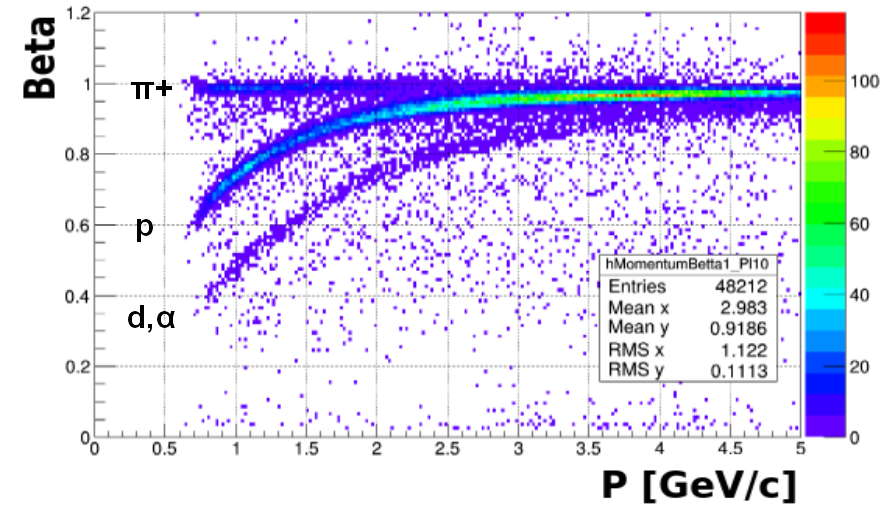
\includegraphics[width=1.\linewidth]{TOF400_PID.png}
      \end{figure}
    \end{block}
    
    \column{.44\textwidth}
    \vskip -.82cm
    \begin{block}{\bf \centering {\scriptsize T = 4.5 GeV/n, C + Cu $\rightarrow$ X}}
      {{\bf \centering \tiny Includes inf. from GEM and DCH trackings}}
      \vskip -.35cm
      \begin{figure}[H]
        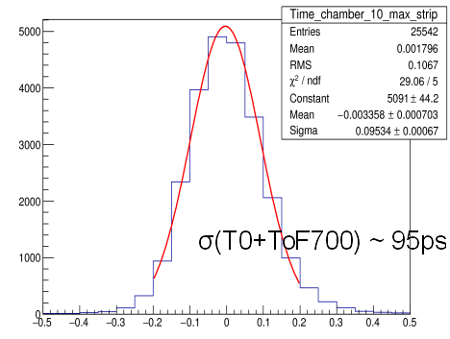
\includegraphics[width=1.\linewidth]{tof700_res.png}
      \end{figure}
      \vskip -.75cm
      \begin{figure}[H]
        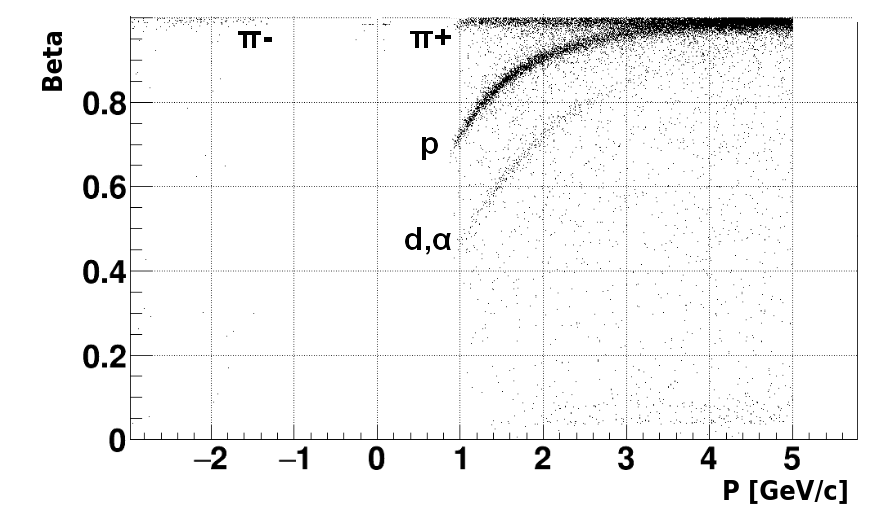
\includegraphics[width=1.\linewidth]{TOF700_PID.png}
      \end{figure}
    \end{block}
  \end{columns}
\end{frame}


\begin{frame}
  \bf
  \begin{block}{}
    \begin{center}
      {\Huge And what about the last run on March 2018?} \\
      {\Huge {\color{red} Data analysis is in progress, but nevertheless...}}
    \end{center}
  \end{block}
\end{frame}

\begin{frame}
  \bf
  \frametitle{\bf \centering Setup \& experimental program to be performed}
  \vskip -.9cm
  % \begin{block}{\bf \centering Setup:}
  \begin{center}
    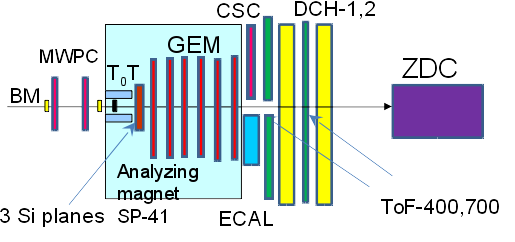
\includegraphics[width=.85\linewidth]{bmn_spring2018_scheme.png}
  \end{center}
 % \end{block}
  \vskip -.9cm
  {\tiny
  \begin{columns}[t]
    \column{.23\textwidth}
    \begin{block}{\bf \centering {\scriptsize Input beams:}}
      Ar beam, $T = 3.2$~AGeV \\
      Kr beam, $T = 2.4, 3.0$~AGeV
    \end{block}
    \column{.33\textwidth}
    \begin{block}{\bf \centering {\scriptsize Aims:}}
      \begin{itemize}
        \item Central tracker inside analyzing magnet $\rightarrow$ 6 GEM detectors $163 \cdot 45 cm^{2}$ and forward Si strip detectors for tracking
        \item Test ToF system, trigger detectors, hadron and EM calorimeters, outer tracker supplemented by CSC
      \end{itemize}
    \end{block} 

    \column{.33\textwidth}
    \begin{block}{\bf \centering {\scriptsize Program:}}
      \begin{itemize}
      \item Measure inelastic reactions Ar (Kr) + target $\rightarrow$ X on targets Al, Cu, Sn, Pb
       % \begin{itemize}
          \item Hyperon production measured in central tracker (Si + GEM)
          \item Charged particles and nuclear fragments identified with ToF
          \item Gamma and multi-gamma states identified in ECAL
        \end{itemize}
        %\end{itemize}
    \end{block}
  \end{columns}
  }
\end{frame}

\begin{frame}
  \bf
  \frametitle{\bf \centering BM@N setup in the last run (before magnet)}
  \vskip -.1cm
  \begin{columns}[t]
    \column{.49\textwidth}
    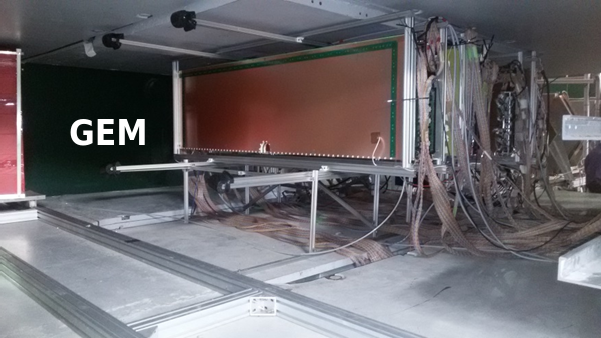
\includegraphics[width=1.\linewidth]{GEMs.png}
    \begin{minipage}{.49\linewidth}
      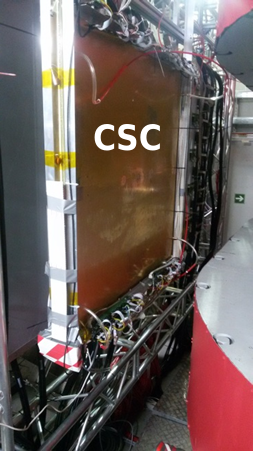
\includegraphics[width=1.\linewidth]{CSC.png}
     % \includegraphics[width=1.\linewidth]{TOF400_installation.png}
    \end{minipage}
    \begin{minipage}{.49\linewidth}
     % \includegraphics[width=1.\linewidth]{CSC.png}
      \includegraphics[width=1.\linewidth]{TOF400_installation.png}
    \end{minipage}

    \column{.49\textwidth}
    \vskip -3.35cm
    \begin{minipage}{1.\linewidth}
      \includegraphics[width=1.\linewidth]{Si_and_Barrel.jpg}
    \end{minipage}
   % \begin{minipage}{.49\linewidth}
   %   \includegraphics[width=1.\linewidth]{DCH1_and_TOF400.jpg}
   % \end{minipage}
    {\footnotesize
    % \begin{minipage}{1.\linewidth}
       \begin{block}{\bf \centering New detector components:}
         \begin{itemize}
         \item Six big GEMs
         \item Trigger detectors
         \item Three Si detectors
         \item CSC chamber
         \item Full set of TOF detectors         
         \end{itemize}
       \end{block}
   %  \end{minipage}
     }
  \end{columns}
\end{frame}

\begin{frame}
  \bf
  \frametitle{\bf \centering BM@N setup in the last run (behind magnet)}
  \begin{minipage}{1.\linewidth}
    \includegraphics[width=1.\linewidth]{detectors_behind_magnet.jpg}
  \end{minipage}
\end{frame}

\begin{frame}
  \bf
  \frametitle{\bf \centering {\footnotesize BM@N and SRC, data collected (March 23 - April 5)}}
  \vskip -.75cm
  \begin{columns}[t]
    \column{.49\textwidth}
    {\scriptsize
    \begin{block}{}
      SRC:
      \begin{itemize}
      \item One beam energy available for C-beam
      \item More than half of the collected statistics can be used for analysis
      \end{itemize}
      BM@N:
      \begin{itemize}
      \item One beam energy available for Ar-beam and three - for Kr-beam
      \item Wide set of targets used ($C, Al, Cu, Sn, Pb$)
      \end{itemize}
    \end{block}
    }
    \column{.50\textwidth}
    \begin{block}{\bf \centering SRC}
     \begin{figure}[H]
      \includegraphics[width=1.\linewidth]{DataCollected_SRC_Run7.eps}
    \end{figure}
    \end{block}
    \vskip -.2cm
     \begin{block}{}
    \begin{center}
      {\color{Red} Data analysis is in progress ...}
    \end{center}
  \end{block}
  \end{columns}
  \vskip -.2cm
  \begin{block}{\bf \centering BM@N}
     \begin{figure}[H]
      \includegraphics[width=1.\linewidth]{DataCollected_BMN_Run7.png}
    \end{figure}
  \end{block}
\end{frame}

\begin{frame}
  \bf
  \frametitle{\bf \centering BM@N beam profile}
  \vskip -.8cm
  \begin{columns}[t]
    \column{.56\textwidth}
    \begin{block}{\bf \centering Beam profiles measured by beam group}
     \resizebox{\columnwidth}{!}{%
       \begin{tabular}{|c| c | c | c |}
         \hline
         & C, Spring 2017 & {\color{red} Ar, Spring 2018} & {\color{red} Kr, Spring 2018} \\
         \hline
         $\sigma_{x} [mm] $ & 6 & {\color{red} 5} & {\color{red} 5.3}\\
         \hline
         $\sigma_{y} [mm] $ & 4.9 & {\color{red} 5} & {\color{red} 3.2}\\
         \hline

       \end{tabular}
       }
    \end{block}
    \vskip -.3cm
     \begin{block}{\bf \centering Kr beam, Y-profile}
       \includegraphics[width=1.\linewidth]{Kr_profileY.jpg}
     \end{block}
        
    \column{.42\textwidth}
    \begin{block}{\bf \centering Kr beam, X-profile}
      \includegraphics[width=1.\linewidth]{Kr_profileX.jpg}
    \end{block}
    \vskip -.3cm
    \begin{block}{}
       \includegraphics[width=1.\linewidth]{bmn_beamZone.png}
    \end{block}   
  \end{columns}
\end{frame}

\begin{frame}
  \bf
  \frametitle{\bf \centering Forward silicon strip detectors}
  \vskip -.75cm
  \begin{columns}[t]
    \column{.3\textwidth}
    \begin{block}{}
      \includegraphics[width=1.\linewidth]{Si_RUN7_1.png}
      \includegraphics[width=1.\linewidth]{Si_RUN7_4.png}
    \end{block}
    \column{.35\textwidth}
    \begin{block}{\bf \centering {\footnotesize Central tracker (GEM + SI) in Argon/Krypton run}}
      \begin{figure}[H]
        \includegraphics[width=1.\linewidth]{Si_RUN7_2.png}
      \end{figure}
    \end{block}
    \vskip -.3cm
    \begin{block}{\bf \centering {\footnotesize Kr beam fragments in silicon vertex detector}}
     \begin{figure}[H]
        \includegraphics[width=1.\linewidth]{Si_RUN7_3.png}
     \end{figure}
     \end{block}
    \column{.30\textwidth} 
    \begin{block}{}
      \begin{itemize}
      \item Two-coordinate Si detector with strip pitch of $95/103 \mu m$, full size of $25 \cdot 25 cm^{2}$ 
      \item Detector consists of 4 sub-detectors located around beam 
      \item 2 smaller vertex detectors (March 2018)
      \end{itemize}
    \end{block}  
  \end{columns}
\end{frame}

\begin{frame}
  \bf
  \frametitle{\bf \centering {\footnotesize New Cathode Strip Chamber (CSC) as Outer tracker}}
  \vskip -.75cm
  \begin{columns}[t]
    \column{.49\textwidth}
    \begin{block}{\bf \centering {\footnotesize Argon (krypton) run:}}
      {\scriptsize CSC chamber installed in front of TOF1 to check its performance as Outer tracker for heavy ions}
      %\end{block}
     
      \begin{center}
        \begin{figure}[H]
          \vskip -.4cm
          \includegraphics[width=.6\linewidth]{CSC_RUN7.png}
        \end{figure}
       \end{center}
    \end{block}
    \column{.49\textwidth}
    \begin{block}{\bf \centering {\tiny Average cluster size:}}
       \includegraphics[width=1.\linewidth]{CSC_clusterSize.png}
    \end{block}
    \vskip -.3cm
    \begin{block}{\bf \centering {\tiny Matching between CSC and DCH:}}
       \includegraphics[width=1.\linewidth]{DCH_CSC_matching.png}
    \end{block}   
  \end{columns}
\end{frame}

\begin{frame}
  \frametitle{\bf \centering {\color{red} Short Range Correlations (SRC)} @ BM@N}
  \begin{center}
    \includegraphics[width=.7\linewidth]{SRC_logo.jpg}
  \end{center}
\end{frame}

\begin{frame}
  \frametitle{\bf \centering How to study SRC?}
  \bf
  \vskip -.75cm
  \begin{columns}[t]
    \column{.49\textwidth}
    \begin{block}{\bf \centering Inverse kinematics}
      \begin{figure}[H]
        \includegraphics[width=1.\linewidth]{src_invKinematics.png}
      \end{figure}
      \vskip -.5cm
      %\end{block}
      %\begin{block}{}
      \ce{^{12}_{6}C} + p $\rightarrow$ 2p + \ce{^{10}_{5}B} + n {\tiny (np SRC)} \\
      \ce{^{12}_{6}C} + p$\rightarrow$ 2p + \ce{^{10}_{4}Be} + p {\tiny (pp SRC)}
    \end{block}
    \vskip -.35cm
           {\scriptsize 
             \begin{block}{\bf \centering Participants}
               \begin{itemize}
               \item JINR: BM@N
                 \vskip -.1cm
               \item Israel: Tel Aviv University
               \item Germany: TUD and GSI
               \item USA: MIT
               \item France: CEA
               \end{itemize}
               \vskip -.55cm
               \begin{figure}[H]
                 \includegraphics[width=1.\linewidth]{all_src_emblems.png}
               \end{figure}
             \end{block}
           }
           

           \column{.49\textwidth}
                  {\footnotesize 
                    \begin{block}{\bf \centering Super exclusive measurement!}
                      Four particles detected:
                      \begin{itemize}
                      \item scattered probe
                      \item knocked-out nucleon
                      \item recoil
                      \item (A-2)-fragment system
                      \end{itemize}
                    \end{block}
                    \vskip -.3cm
                    \begin{block}{\bf \centering Objectives}
                      \begin{itemize}
                      \item identifying 2N-SRC events with inverse kinematics
                      \item studying isospin decomposition of 2N-SRC
                      \item studying (A-2) spectator nuclear system
                      \end{itemize}
                    \end{block}
                    \vskip -.3cm  
                    \begin{block}{}
                      \vskip -.1cm
                             {\color{Red} First BM@N SRC program run in March 2018: $\sim$ 30 MEvents collected}
                    \end{block}
                  }
  \end{columns}
\end{frame}

\begin{frame}
  \frametitle{\bf \centering Experimental setup}
  \vskip -.25cm
  \begin{block}{}
    \vskip -.3cm
    \begin{figure}[H]
      \includegraphics[width=1.\linewidth]{src_setup.png}
    \end{figure}
  \end{block}
\end{frame}

\begin{frame}
  \frametitle{\bf \centering Counter analysis (A - 2) identification}
  \vskip -.75cm
  \begin{columns}[t]
     \column{.44\textwidth}
    \begin{block}{\bf \centering {\scriptsize Before target:}}
      \includegraphics[width=1.\linewidth]{src_sepbeforeTarget.png}
    \end{block}
    \vskip -.3cm
    \begin{block}{\bf \centering {\scriptsize After target:}}
      \includegraphics[width=1.\linewidth]{src_sepAfterTarget.png}
    \end{block}
    \column{.51\textwidth}
    \begin{block}{\bf \centering {\footnotesize Nuclear fragment identification}}
      \includegraphics[width=1.\linewidth]{src_FragmentIdentif.png}
      \includegraphics[width=1.\linewidth]{src_FragmentIdentif_2.png}
    \end{block}  
  \end{columns}
\end{frame}

\begin{frame}
  \bf
  \frametitle{\bf \centering BM@N: past \& future, status \& plans}
  \vskip -.25cm
  \begin{block}{\bf \centering Beam parameters and setup at different stages of the experiment}
    \resizebox{\columnwidth}{!}{%
      \begin{tabular}{| c | c | c | c | c | c|}
        \hline
        Year & {\color{Blue} 2016} & {\color{Blue} 2017} & {\color{Blue} 2018} & {\color{Red} 2020} & {\color{Red} 2021 and later} \\
        \hline
        Experim. status & {\color{Blue} techn. run} & {\color{Blue} techn.run} & {\color{Blue} techn. run} & {\color{Red} stage 1, phys.} &
        {\color{Red} stage 2, phys.} \\
        \hline
        Beam & {\color{Blue} d($\uparrow$)} & {\color{Blue} C} & {\color{Blue} Ar, Kr, C} & {\color{Red} Au} & {\color{Red} p, Au} \\
        \hline
        Max. intensity [MHz] & {\color{Blue} 0.5} & {\color{Blue} 0.5} & {\color{Blue} 0.5} & {\color{Red} 1} & {\color{Red} 10} \\
        \hline
        Trigger rate [kHz] & {\color{Blue} 5} & {\color{Blue} 5} & {\color{Blue} 10} & {\color{Red} 10} & {\color{Red} 20-50} \\
        \hline
        \multicolumn{6}{|c|}{Central tracker} \\
        \hline
        GEM & {\color{Blue} 6 (half planes)} & {\color{Blue} 6 (half planes)} & {\color{Blue} 6 (half planes)} & {\color{Red} 7} & {\color{Red} 7} \\
        \hline
        SI & {\color{Blue} -} & {\color{Blue} 1 (small plane)} & {\color{Blue} 3 (small planes)} & {\color{Red} 4} & {\color{Red} 4} \\      
        \hline
      \end{tabular}
    }
  \end{block}
  \begin{columns}[t]
    \column{.49\textwidth}
    \vskip -.75cm
           {\color{Blue} \tiny 
             \begin{block}{\bf \centering Status:}
               \vskip .2cm
               \begin{itemize}
               \item Technical runs with deuteron and carbon beams (T = 3.5 - 4.6 GeV/n), argon beam (T = 3.2 GeV/n) and krypton beam (T = 2.3 GeV/n) performed
               \item Measurement on Short Range Correlations with inverse kinematics: C + $H_{2}$-target performed
               \item Major sub-systems are operational, but are still in limited configurations: GEMs, forward Silicon detectors, Outer tracker, ToF, ZDC, ECAL,
                 trigger, DAQ, slow control, online monitoring
               \item Аlgorithms for event reconstruction and analysis are being developed
               \end{itemize}      
             \end{block}
           }
           \column{.49\textwidth}
           \vskip -.75cm
                  {\color{Red} \scriptsize
                    \begin{block}{\bf \centering Plans:}
                      \begin{itemize}
                      \item Collaborate with CBM to produce and install large aperture silicon detectors in front of GEM-tracker
                      \item Extend the GEM central tracker and the CSC outer tracker to full configuration
                      \item Implement beam detectors into vacuum beam pipe, implement vacuum / helium beam pipe through the BM@N setup
                      \end{itemize}
                    \end{block}
                  }
  \end{columns}
\end{frame}

\begin{frame}
  \bf
  \frametitle{\bf \centering Conclusion:}
  \begin{itemize}
  \item BM@N experiment has recorded experimental data with carbon, argon and krypton beams at several energies and on several targets.
  \item Minimum bias interactions have been analyzed aimed to reconstruct tracks, primary and secondary vertices using central GEM and Si tracking detectors.
  \item Reconstructed signals of $\Lambda^{0}$ and $K^{0}_{s}$ are visible in proton-pion and pion-pion invariant mass spectra.
  \item 
  \end{itemize}
\end{frame}

\begin{frame}
  \frametitle{\bf \centering Towards realistic simulation of GEM tracker}
  \vskip -.25cm
  \begin{block}{}
    \begin{center}
      \bf {\footnotesize Simulation of GEM response: Garfield++}
    \end{center}
  \end{block}
  \vskip -.75cm
  \begin{columns}[t]
    \column{.49\textwidth}
    {\scriptsize
    \begin{block}{}
      \bf
      \begin{itemize}
        \item {\color{red} Garfield++} is a framework for micro-simulation of physical processes in gas detectors 
        \item A charge particle passing through GEM chamber detecting volume ionizes electrons in gas  
        \item Multiplayer GEM-cascades form avalanches which drift to readout-plane and fire strips
      \end{itemize}
    \end{block}
    }
    \vskip -.4cm
    \begin{block}{\bf \centering {\scriptsize Simulation parameters in Garfield++}}
      \includegraphics[width=1.\linewidth]{GEM_internStruct.png} 
    \end{block}
    \column{.49\textwidth}
    \begin{block}{\bf \centering {\scriptsize Structure of BM@N GEM chamber and simulated electron avalanches}}
      \includegraphics[width=1.\linewidth]{GEM_electronAvalanche.png} 
    \end{block}
    \vskip -.3cm
    \begin{block}{\bf \centering {\scriptsize Profile of electron avalanche at the readout-plane (cluster)}}
      \includegraphics[width=1.\linewidth]{GEM_electronAvProfile.png} 
    \end{block}
  \end{columns} 
\end{frame}


\end{document}
